\documentclass{article}
\usepackage[utf8]{inputenc}
\usepackage{graphicx}
\usepackage[spanish,es-tabla]{babel}
\usepackage{amsmath}
\usepackage[a4paper,margin=1in]{geometry}
\usepackage{subcaption}
\usepackage{amssymb}
\usepackage[hidelinks]{hyperref}
\usepackage{mathtools}
\usepackage[table,xcdraw]{xcolor}
\usepackage[style=ieee, backend=biber]{biblatex}
\usepackage{enumitem}
\usepackage{csquotes}
\usepackage{circuitikz}
\graphicspath{{Figuras/}}           
\addbibresource{bibliografía.bib}   
\hypersetup{
    colorlinks=true,
    linkcolor=blue,    
    citecolor=blue,
    urlcolor=blue,
    filecolor=blue
}


\begin{document}       
\renewcommand{\figureautorefname}{Fig.}
\renewcommand{\tableautorefname}{Tab.}
\renewcommand{\equationautorefname}{Ec.}


\begin{titlepage}
\thispagestyle{empty}
\begin{tikzpicture}[remember picture,overlay]
    \node[opacity=0.2,anchor=center] at (current page.center) 
        {
\includegraphics[width=0.9\paperwidth]{decoracion_a.png}};
\end{tikzpicture}
\begin{center}
    
\includegraphics[width=15cm]{unc_fcefyn_logo.png} \\ [0.5cm]
    \LARGE Universidad Nacional de Córdoba \\ [0.5cm] 
    \large Facultad de Ciencias Exactas, Físicas y Naturales \\ [0.5cm] 
    \large Electrónica Analógica III \\ [0.2cm]
    \large Trabajo Práctico N°2 \\ [0.2cm]
    \vspace{60pt}
    \begin{table}[!h]
        \centering
        \begin{tabular}{ll}
            \multicolumn{1}{c}{Nombre} & \multicolumn{1}{c}{DNI} \\
            Dávila Tomassi, Carlos Valentino & 40.000.000 \\
            Mendes Rosa, Agustín             & 44.517.201 \\
            Monja, Ernesto Joaquín           & 43.873.728
        \end{tabular}
    \end{table}
    \vspace{20pt}
    \begin{table}[!h]
        \centering
        \begin{tabular}{ll}
            \multicolumn{1}{c}{Docentes} & Ing. Bruni, Rodrigo Gabriel \\
                                         & Ing. Dadam, Federico Tomás \\
        \end{tabular}
    \end{table}
    \vfill
        Córdoba, República Argentina\\
        Año 2026
\end{center}
\end{titlepage}
\newpage

\tableofcontents
\newpage
\indent

\section{Introducción y objetivos} \label{section:sec_1}
En el presente informe se detalla el procedimiento de cálculo, simulación, implementación y medición de un amplificador de bajo ruido (LNA, por sus siglas en inglés) clase A para señales de microondas. 

El diseño se basa en el transistor bipolar de heterounión (BJT) modelo BFP760. Se emplea una frecuencia de trabajo de $\mathrm{2 \ GHz}$ y se considera una impedancia característica del sistema de $\mathrm{50 \ \Omega}$ ($\mathrm{Z_{0} = Z_{L} = Z_{S} = 50 \ \Omega}$). El amplificador es tratado como una red bilateral, requiriendo una adaptación simultánea conjugada en los puertos de entrada y salida mediante el uso de líneas de transmisión tipo \textit{microstrip}.

Para el desarrollo del trabajo práctico se plantearon los siguientes objetivos particulares:
\begin{itemize}
    \item Definir un punto de polarización en corriente continua que garantice estabilidad incondicional, máxima ganancia y mínimo ruido.
    \item Calcular las redes de adaptación de impedancia de entrada y salida utilizando tecnología \textit{microstrip}.
    \item Simular el circuito diseñado evaluando parámetros de dispersión o ``$\mathrm{S}$'' (por ``\textit{scattering}'') e indicadores de desempeño en entornos ideales y con modelos físicos.
    \item Fabricar el circuito impreso (PCB) incorporando las redes de polarización y adaptación.
    \item Medir los parámetros de desempeño del prototipo empleando el instrumental adecuado y contrastar los resultados físicos con los teóricos y simulados.
\end{itemize}

\newpage

\section{Marco Teórico} \label{sec_2}
\subsection{Low Noise Amplifier (LNA)} \label{section:sec_2.1}
El objetivo de estos dispositivos es amplificar señales de RF de baja potencia tomadas de una antena hasta el nivel requerido por las etapas consecuentes, minimizando el valor de figura de ruido \cite{bose_lna}. Debido a esto es que se utiliza como primer bloque en un receptor de RF (véase \autoref{fig:Receptor}), ya que sus características tienen mayor influencia que los demás bloques en la figura de ruido total, tal como lo muestra la \autoref{eq:NF}, donde $\mathrm{F_{i}}$ es la figura de ruido y $\mathrm{G_{i}}$ la ganancia del sistema $\mathrm{i}$.

\begin{equation}
    \mathrm{F_{T} = F_{1} + \frac{F_{2} - 1}{G_{1}} + \frac{F_{3} - 1}{G_{1}G_{2}} + \dots + \frac{F_{N} - 1}{\prod_{i=1}^{N-1}G_{i}}}
    \label{eq:NF}
\end{equation}

\begin{figure}[!h]
    \centering
    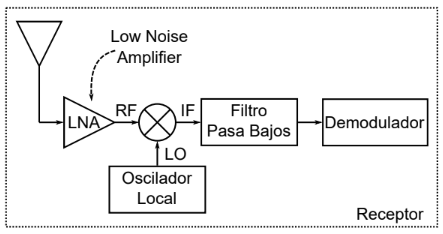
\includegraphics[width=0.5\textwidth]{Figuras/Receptor.png}
    \caption{Esquemático receptor de RF.}
    \label{fig:Receptor}
\end{figure}

\subsection{Microtiras} \label{section:sec_2.2}
Son un tipo de línea de transmisión, que debido a su facilidad de fabricación en PCB se utilizan ampliamente en amplificadores de RF \cite[págs.~141--147]{gonzalez_amplifiers}. El sustrato sobre el cual se trazan las microtiras se caracteriza según el valor de: 
\begin{itemize}
    \item Altura del dieléctrico ($\mathrm{h}$)
    \item Espesor del cobre ($\mathrm{t}$)
    \item Permitividad eléctrica ($\mathrm{\epsilon_{r}}$)
\end{itemize}

El comportamiento de la microtira y su impedancia característica ($\mathrm{Z_0}$) depende de éstos parámetros, junto con el ancho de la tira ($\mathrm{W}$) y la longitud de la misma ($\mathrm{d}$). Notar que en la \autoref{fig:Geometria_microtira} pueden verse algunos de los parámetros mencionados.
\begin{figure}[!h]
    \centering
    \fbox{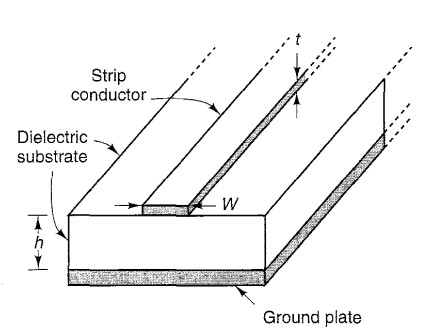
\includegraphics[width=0.5\textwidth]{Figuras/Microstrips.png}}
    \caption{Geometría de una microtira.}
    \label{fig:Geometria_microtira}
\end{figure}

Para sintetizar una microtira según un $\mathrm{Z_{0}}$ requerido, se deben determinar $\mathrm{W}$ y $\mathrm{d}$ utilizando las ecuaciones de Hammerstad. Con ellas se calculan los factores $\mathrm{A}$ y $\mathrm{B}$ (\autoref{eq:A} y \autoref{eq:B}), y con ellos la relación geométrica $\mathrm{\frac{W}{h}}$ para obtener $\mathrm{W}$ sabiendo el valor de $\mathrm{h}$ (véase la \autoref{eq:W_H}). 
\begin{equation}
    \mathrm{A = \frac{Z_{0}}{60} \sqrt{\frac{\epsilon_{r} + 1}{2}} + \frac{\epsilon_{r} - 1}{\epsilon_{r} + 1} \left(0.23 + \frac{0.11}{\epsilon_{r}} \right)}
    \label{eq:A}
\end{equation}

\begin{equation}
    \mathrm{B = \frac{377 \cdot \pi}{2 \cdot Z_{0} \cdot \sqrt{\epsilon_{r}}}}
    \label{eq:B}
\end{equation}

\begin{equation}
    \mathrm{\frac{W}{h} =} 
    \begin{cases} 
        \mathrm{\dfrac{8  \cdot e^{A}}{e^{2A} - 2}} & \text{para } \mathrm{\frac{W}{h} \leq 2} \\ 
        \\
        \mathrm{\dfrac{2}{\pi} \left[ B - 1 - \ln(2B - 1) + \dfrac{\epsilon_{r} - 1}{2\epsilon_{r}} \left( \ln(B - 1) + 0.39 - \dfrac{0.61}{\epsilon_{r}} \right) \right]} & \text{para } \mathrm{\frac{W}{h} \geq 2} 
    \end{cases}
    \label{eq:W_H}
\end{equation} \\

Que el espesor del cobre ($\mathrm{t}$) sea finito implica la aparición de un efecto de primer orden que aumenta la capacitancia, por lo que puede compensarse corrigiendo el ancho de la tira según la \autoref{eq:weff}.
\begin{equation}
    \mathrm{W_{eff} = }
    \begin{cases} 
        \mathrm{W + \dfrac{t}{\pi} \cdot \left[ 1 + \ln\left( \dfrac{4\pi W}{t} \right) \right]} & \text{para } \mathrm{\frac{W}{h} \leq \dfrac{1}{2\pi}} \\ 
        \mathrm{W + \dfrac{t}{\pi} \cdot \left[ 1 + \ln\left( \dfrac{2h}{t} \right) \right]} & \text{para } \mathrm{\frac{W}{h} \geq \dfrac{1}{2\pi}}
    \end{cases}
    \label{eq:weff}
\end{equation} \\

Por último, debido a que parte de las lineas de campo están en el área del dieléctrico y otras en el aire, se define la permitividad eléctrica efectiva ($\mathrm{\epsilon_{eff}}$) aplicando la corrección que muestra la \autoref{eq:eff}.
\begin{equation}
    \mathrm{\epsilon_{eff} =}
    \begin{cases} 
        \mathrm{\frac{\epsilon_{r} + 1}{2} + \frac{\epsilon_{r} - 1}{2} \cdot \left[ \frac{1}{\sqrt{1 + \frac{12 \cdot h}{W}}} +0.04 \left( 1 - \frac{W}{h}\right)^2\right]} & \text{para } \mathrm{\frac{W}{h} \leq 1} \\ 
        \mathrm{\frac{\epsilon_{r} + 1}{2} + \frac{\epsilon_{r} - 1}{2} \cdot \frac{1}{\sqrt{1 + \frac{12 \cdot h}{W}}} } & \text{para } \mathrm{\frac{W}{h} \geq 1}
    \end{cases}
    \label{eq:eff}
\end{equation} \\



\subsection{Parámetros de dispersión (S)} \label{section:sec_2.3}
Para el análisis de circuitos en altas frecuencias, donde las dimensiones físicas son comparables a la longitud de onda, se utilizan los parámetros ``$\mathrm{S}$'' \cite[págs.~23--24]{gonzalez_amplifiers}. Estos relacionan las ondas de tensión incidentes ($\mathrm{a_n}$) y reflejadas ($\mathrm{b_n}$) en los puertos de la red, también llamadas ``pseudowaves''. 

Para un dispositivo de dos puertos, la relación se define en la \autoref{eq:param_s}, donde $\mathrm{S_{11}}$ y $\mathrm{S_{22}}$ representan los coeficientes de reflexión en la entrada y salida, mientras que $\mathrm{S_{21}}$ y $\mathrm{S_{12}}$ representan la ganancia directa y el aislamiento inverso, respectivamente, según indica la \autoref{fig:Param_S}.
\begin{equation}
    \begin{bmatrix} \mathrm{b_{1}} \\ \mathrm{b_{2}} \end{bmatrix} = 
    \begin{bmatrix} \mathrm{S_{11}} & \mathrm{S_{12}} \\ \mathrm{S_{21}} & \mathrm{S_{22}} \end{bmatrix} 
    \begin{bmatrix} \mathrm{a_{1}} \\ \mathrm{a_{2}} \end{bmatrix}
    \label{eq:param_s}
\end{equation}

\begin{figure}[!h]
    \centering
    \fbox{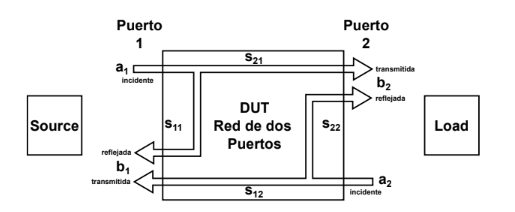
\includegraphics[width=0.65
    \linewidth]{Param_S.png}}
    \caption{Diagrama para una red de 2 puertos}
    \label{fig:Param_S}
\end{figure}

Según la \autoref{fig:Coefs}, es posible definir los coeficientes de reflexión en términos de las pseudowaves y de las impedancias vistas en el circuito, con tal de poder relacionarlas con los valores de los parámetros $\mathrm{S}$ (\autoref{eq:Gamma_S}, \autoref{eq:Gamma_L}, \autoref{eq:Gamma_in}, \autoref{eq:Gamma_out}) \cite[p.~214]{gonzalez_amplifiers}. Notar que si se adaptan las impedancias del circuito (es decir, $\mathrm{Z_{S} = Z_{L} =Z_{0}}$), los coeficientes $\mathrm{\Gamma_{L}}$ y $\mathrm{\Gamma_{S}}$ se reducen a cero y no hay ondas reflejadas de vuelta al amplificador.
\begin{equation}
    \mathrm{\Gamma_{S} = \frac{a_{1}}{b_{1}} = \frac{Z_{S} - Z_{0}}{Z_{S} + Z_{0}}}
    \label{eq:Gamma_S}
\end{equation}

\begin{equation}
    \mathrm{\Gamma_{L} = \frac{a_{2}}{b_{2}} = \frac{Z_{L} - Z_{0}}{Z_{L} + Z_{0}}}
    \label{eq:Gamma_L}
\end{equation}

\begin{equation}
    \mathrm{\Gamma_{in} = \frac{b_{1}}{a_{1}} = S_{11} + \frac{S_{12}S_{21}\Gamma_L}{1 - S_{22}\Gamma_{L}}}
    \label{eq:Gamma_in}
\end{equation}

\begin{equation}
    \mathrm{\Gamma_{out} = \frac{b_{2}}{a_{2}} = S_{22} + \frac{S_{12}S_{21}\Gamma_S}{1 - S_{11}\Gamma_{S}}}
    \label{eq:Gamma_out}
\end{equation}

\begin{figure}[!h]
    \centering
    \fbox{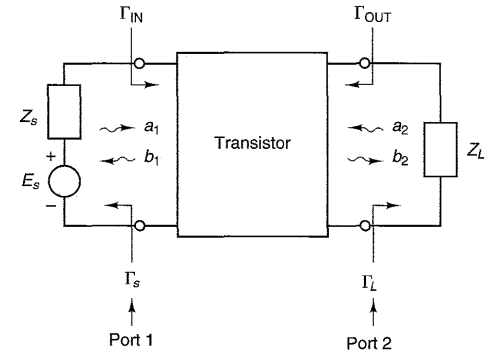
\includegraphics[width=0.5\linewidth]{Figuras/Coef_Reflexion.png}}
    \caption{Diagrama de bloques de un amplificador de microondas.}
    \label{fig:Coefs}
\end{figure}



\subsection{Ganancia para redes de 2 puertos} \label{section:sec_2.4}
Considerando una red de dos puertos, caracterizada por una matriz $\mathrm{[S]}$ y conectada a una fuente y una carga como se ve en la \autoref{fig:Coefs}, se tienen tres tipos de ganancia que pueden expresarse en términos de los parámetros $\mathrm{S}$ \cite[p.~559]{pozar_microwave}:
\begin{itemize}
    \item \underline{Transductance Power Gain ($\mathrm{G_{T}}$)}: Ganancia total de la entrada a la salida. (\autoref{eq:GT}).
    \begin{equation}
        \mathrm{G_{T} = \frac{P_{L}}{P_{AV(S)}} = \frac{1 - |\Gamma_{S}|^{2}}{|1 - \Gamma_{in} \Gamma_{S}|^{2}} \cdot |S_{21}|^{2} \cdot \frac{1 - |\Gamma_{L}|^{2}}{|1 - S_{22}\Gamma_{L}|^{2}}}
        \label{eq:GT}
    \end{equation}
    
    \item \underline{Operating Power Gain ($\mathrm{G_{P}}$)}: Ganancia entregada a la carga según cuánto entró al DUT. (\autoref{eq:GP}).
    \begin{equation}
        \mathrm{G_{P} = \frac{P_{L}}{P_{in}} = \frac{1}{1 - |\Gamma_{in}|^{2}} \cdot |S_{21}|^{2} \cdot \frac{1 - |\Gamma_{L}|^{2}}{|1 - S_{22}\Gamma_{L}|^{2}}}
        \label{eq:GP}
    \end{equation}
    
    \item \underline{Available Power Gain ($\mathrm{G_{A}}$)}: Ganancia disponible en el segundo puerto según cuánto entrega la fuente. (\autoref{eq:GA}).
    \begin{equation}
        \mathrm{G_{A} = \frac{P_{AV(N)}}{P_{AV(S)}} = \frac{1 - |\Gamma_{S}|^{2}}{|1 - S_{11}\Gamma_{S}|^{2}} \cdot |S_{21}|^{2} \cdot \frac{1}{1 - |\Gamma_{out}|^{2}}}
        \label{eq:GA}
    \end{equation}
\end{itemize}

Para obtener la ganancia máxima posible, no alcanza con adaptar la entrada y salida la impedancia del sistema (es decir, $\mathrm{\Gamma_{S} = \Gamma_{L} = 0}$), debido a que los coeficientes $\mathrm{S_{11}}$ y $\mathrm{S_{22}}$ del transistor propio son distintos de 0. Esta condición genera que la $\mathrm{G_{T}}$ de la red sea igual a la del transistor ($\mathrm{|S_{21}|^{2}}$).

La maximización de ganancia se logra utilizando la adaptación conjugada simultánea, descrita en la \autoref{section:sec_2.5}.
\\


\subsection{Adaptación conjugada simultánea} \label{section:sec_2.5} 
Este tipo de adaptación consta de adaptar la impedancia de la fuente y la carga tal que se transformen en $\mathrm{\Gamma_{in}^*}$ y $\mathrm{\Gamma_{out}^*}$ respectivamente para el transistor (\autoref{eq:conjugado}). Éste ve hacia la red el conjugado exacto de su propia impedancia y así toda la potencia disponible del generador ingresa al transistor, y toda la potencia disponible del transistor se entrega a la carga, por eso se aplica cuando se desea maximizar la ganancia de la entrada a la salida (\autoref{eq:GTmax}).

\begin{equation}
    \begin{aligned}
        \mathrm{Z_{in}}  & \mathrm{= Z_{S}^{*} \;\Rightarrow\; \Gamma_{in}  = \Gamma_{S}^{*}} \\
        \mathrm{Z_{out}} & \mathrm{= Z_{L}^{*} \;\Rightarrow\; \Gamma_{out} = \Gamma_{L}^{*}} 
    \end{aligned}
    \label{eq:conjugado}
\end{equation}
\\

\begin{equation}
    \mathrm{G_{T(max)} = \frac{1}{1 - |S_{11}|^2} \cdot |S_{21}|^2 \cdot \frac{1}{1 - |S_{22}|^2} = G_{P(max)} = G_{A(max)}}
    \label{eq:GTmax}
\end{equation}
\\



\subsection{Estabilidad} \label{section:sec_2.6}
Un amplificador puede volverse inestable si el puerto de entrada o salida tiene parte real negativa, implicando que $\mathrm{|\Gamma_{in}| > 1}$ o $\mathrm{|\Gamma_{out}| > 1}$. Debido a que éstos dependen de las redes de adaptación de la fuente y la carga, la estabilidad del amplificador depende de $\mathrm{\Gamma_{S}}$ y $\mathrm{\Gamma_{L}}$ \cite[págs.~564--568]{pozar_microwave}. A partir de esto pueden presentarse dos tipos de estabilidad:

\begin{itemize}
    \item \underline{Estabilidad incondicional}: Se cumple si $\mathrm{|\Gamma_{in}| < 1}$ y $\mathrm{|\Gamma_{out}| < 1}$ para todas las impedancias pasivas de fuente y carga (es decir, $\mathrm{|\Gamma_{L}| < 1}$ y $\mathrm{|\Gamma_{S}| < 1}$).

    \item \underline{Estabilidad condicional:} Se cumple si $\mathrm{|\Gamma_{in}| < 1}$ y $\mathrm{|\Gamma_{out}| < 1}$ solo para un rango específico de impedancias pasivas de fuente y carga.
\end{itemize}

Para analizar el rango de valores de $\mathrm{\Gamma_{L}}$ y $\mathrm{\Gamma_{S}}$ donde el amplificador es estable, se deben trazar los círculos de estabilidad de entrada (\autoref{eq:C_in}) y de salida (\autoref{eq:C_out}) en la Carta de Smith. La zona de operación estable para la entrada será el área que encierra el círculo de estabilidad de entrada, mientras que para la salida será el área que queda por fuera del círculo de estabilidad de salida.

\begin{equation}
    \begin{aligned}
        \mathrm{C_{S}} & \mathrm{= \frac{(S_{11} - \Delta S_{22}^{*})^{*}}{|S_{11}|^{2} - |\Delta|^{2}}} & \text{(centro),}\\
        \mathrm{R_{S}} & \mathrm{= \left| \frac{S_{12}S_{21}}{|S_{11}|^{2} - |\Delta|^{2}} \right|} & \text{(radio).}
    \end{aligned}
    \label{eq:C_in}
\end{equation}
\\

\begin{equation}
    \begin{aligned}
        \mathrm{C_{L}} & \mathrm{= \frac{(S_{22} - \Delta S_{11}^{*})^{*}}{|S_{22}|^{2} - |\Delta|^{2}}} & \text{(centro),}\\
        \mathrm{R_{L}} & \mathrm{= \left| \frac{S_{12}S_{21}}{|S_{22}|^{2} - |\Delta|^{2}} \right|} & \text{(radio).}
    \end{aligned}
    \label{eq:C_out}
\end{equation}
\\

La estabilidad incondicional del sistema puede evaluarse rápidamente aplicando criterio de Rollet, que establece las condiciones que describe la \autoref{eq:cond} para dos parámetros, el factor de estabilidad ($\mathrm{k}$. Ver \autoref{eq:rollet}) y el determinante de la matriz $\mathrm{[S]}$ ($\mathrm{\Delta}$. Ver \autoref{eq:Delta}).

\begin{equation}
    \begin{cases}
        \mathrm{k > 1} \\
        \mathrm{|\Delta| < 1}
    \end{cases}
    \label{eq:cond}
\end{equation}

\begin{equation}
    \mathrm{k = \frac{1 - |S_{11}|^{2} - |S_{22}|^{2} + |\Delta|^{2}}{2 |S_{12} S_{21}|}}    
    \label{eq:rollet}
\end{equation}

\begin{equation}
    \mathrm{\Delta = S_{11}S_{22} - S_{12}S_{21}}
    \label{eq:Delta}
\end{equation}
\\

Si no se cumple con la estabilidad incondicional, no es posible aplicar la adaptación conjugada simultánea para extraer la máxima ganancia del dispositivo, sino que se deben trazar los círculos de estabilidad de entrada y salida, y elegir un punto de operación que garantice un comportamiento estable. 

En este caso, la ganancia máxima a la que puede apuntarse puede calcularse como una figura de mérito (MSG, Maximum Stable Gain) según la ecuación \autoref{eq:MSG} \cite[p.~572]{pozar_microwave}.

\begin{equation}
    \mathrm{MSG = \frac{|S_{21}|}{|S_{12}|}}
    \label{eq:MSG}
\end{equation}
\\



\subsection{Características del transistor} \label{section:sec_2.7}
Se puede utilizar el modelo serie de impedancias de un BJT que muestra la \autoref{fig:mod_serie} a partir del cálculo de los coeficientes de reflexión, que varía según el tipo de estabilidad del amplificador.

\begin{figure}[!h]
    \centering
    \fbox{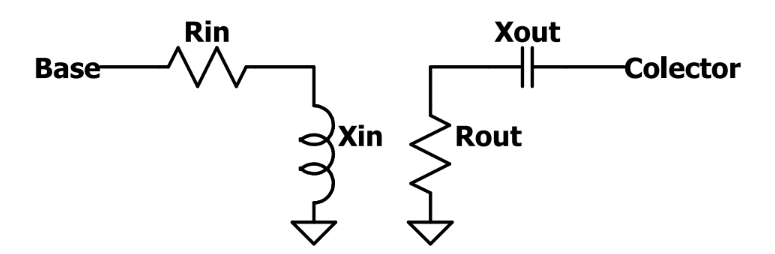
\includegraphics[width=0.5\linewidth]{Figuras/Mod_serie.png}}
    \caption{Modelo de BJT con impedancias serie.}
    \label{fig:mod_serie}
\end{figure}



\subsubsection{Caso para estabilidad incondicional} \label{section:sec_2.7.1}
Se aplica la adaptación conjugada simultánea según \autoref{eq:coefs_1} y \autoref{eq:coefs_2} \cite[p.~572]{pozar_microwave}.
\begin{equation}
    \begin{aligned}
        \mathrm{\Gamma_{S(m)} = \Gamma_{in}^{*}}  & \mathrm{= \frac{B_{1} - \sqrt{B_{1}^{2} - 4|C_{1}|^{2}}}{2C_{1}}}  \\
        \mathrm{\Gamma_{L(m)} = \Gamma_{out}^{*}} & \mathrm{= \frac{B_{2} - \sqrt{B_{2}^{2} - 4|C_{2}|^{2}}}{2C_{2}}}
    \end{aligned}
    \label{eq:coefs_1}
\end{equation}

\begin{equation}
    \begin{cases}
        \mathrm{B_{1}} & \mathrm{= 1 + |S_{11}|^{2} - |S_{22}|^{2} - |\Delta^{2}|} \\
        \mathrm{B_{2}} & \mathrm{= 1 + |S_{22}|^{2} - |S_{11}|^{2} - |\Delta^{2}|} \\
        \mathrm{C_{1}} & \mathrm{= S_{11} - (\Delta S_{22}^{*})} \\
        \mathrm{C_{2}} & \mathrm{= S_{22} - (\Delta S_{11}^{*})}
    \end{cases}
    \label{eq:coefs_2}
\end{equation}
\\

\subsubsection{Caso para estabilidad condicional} \label{section:sec_2.7.2}
Se traza el círculo de estabilidad de salida en la Carta de Smith y se elige un valor de $\mathrm{\Gamma_L}$ dentro de la zona estable. Luego a partir de ese valor se calcula $\mathrm{\Gamma_{in}}$ según la \autoref{eq:Gamma_in} y posteriormente se obtiene $\mathrm{\Gamma_S}$ aplicando el conjugado a $\mathrm{\Gamma_{in}}$. Debe verificarse, según el circulo de estabilidad de entrada, que éste también caiga en zona estable.

Por último se utiliza $\mathrm{\Gamma_S}$ para calcular $\mathrm{\Gamma_{out}}$ según la \autoref{eq:Gamma_out} \cite[p.~252]{gonzalez_amplifiers}.
\\

\subsubsection{Cálculo de impedancias} \label{section:sec_2.7.3}
Obtenidos los valores de los coeficientes de reflexión, es posible calcular $\mathrm{Z_{in}}$ y $\mathrm{Z_{out}}$ según la \autoref{eq:Ztransistor}, dependiendo del valor de $\mathrm{Z_0}$ \cite[p.~59]{pozar_microwave}. 

Se puede cambiar a un modelo paralelo equivalente de las impedancias según la \autoref{eq:serie_a_paralelo} \cite[p.~125]{gonzalez_amplifiers}.

\begin{equation}
    \begin{aligned}
        \mathrm{Z_{in}}  & \mathrm{= Z_0 \ \frac{1 + \Gamma_{in}}{1 - \Gamma_{in}}} \\
        \mathrm{Z_{out}} & \mathrm{= Z_0 \ \frac{1 + \Gamma_{out}}{1 - \Gamma_{out}}}
    \end{aligned}
    \label{eq:Ztransistor}
\end{equation}

\begin{equation}
    \label{eq:serie_a_paralelo}
    \begin{cases} 
        \mathrm{R_{in(p)} = R_{in(s)} \left[1 + \left( \dfrac{X_{in(s)}}{R_{in(s)}} \right)^2 \right]} \\[15pt]
        \mathrm{X_{in(p)} = X_{in(s)} \left[ 1 + \left( \dfrac{R_{in(s)}}{X_{in(s)}} \right)^2 \right]}
    \end{cases}
\end{equation}
\\



\subsection{Adaptación de impedancias mediante líneas de transmisión} \label{section:sec_2.8}
En frecuencias de microondas, los componentes concentrados comerciales presentan pérdidas severas por radiación y efectos parásitos ya que sus dimensiones físicas son comparables con la longitud de onda, por lo que se recurre al uso de microtiras para sintetizar elementos reactivos y realizar redes de transformación de impedancia \cite[págs.~59--62]{pozar_microwave}.

La impedancia de entrada $\mathrm{Z(d)}$ vista a una distancia física $\mathrm{d}$ desde la carga en una línea de transmisión con impedancia característica $\mathrm{Z_0}$, y cargada con una impedancia genérica $\mathrm{Z_L}$, se determina mediante la ecuación descrita en la \autoref{eq:Z_linea}.
\begin{equation}
    \mathrm{Z(d) = Z_{0} \cdot \left[ \frac{Z_{L} + j Z_{0} \cdot \tan(\beta \cdot d)}{Z_{0} + j Z_{L} \cdot \tan(\beta \cdot d)} \right]}
    \label{eq:Z_linea}
\end{equation}
Donde $\mathrm{\beta}$ representa la constante de fase de la línea de transmisión.



\subsubsection{Transformador de un cuarto de longitud de onda ($\lambda/4$)} \label{section:sec_2.8.1}
El transformador de $\lambda/4$ consiste en una sección de línea de transmisión de longitud eléctrica igual a $90^\circ$ ($\beta \cdot \mathrm{d} = \pi/2$). Al evaluar esta condición en la \autoref{eq:Z_linea} la expresión se simplifica analíticamente permitiendo obtener una impedancia de entrada deseada según lo establece la \autoref{eq:lambda_cuarto}.
\begin{equation}
    \mathrm{Z_{in} = \frac{Z_{m}^{2}}{Z_{L}}}
    \label{eq:lambda_cuarto}
\end{equation}

De esta manera, para adaptar una impedancia real hacia el valor del sistema, la impedancia característica de la microtira adaptadora ($\mathrm{Z_m}$) debe calcularse como la media geométrica indicada en la \autoref{eq:Z_m_calc}.
\begin{equation}
    \mathrm{Z_m = \sqrt{Z_{in} \cdot Z_{L}}}
    \label{eq:Z_m_calc}
\end{equation}
\\



\subsubsection{Síntesis de elementos reactivos en paralelo} \label{section:sec_2.8.2}
Cuando una línea de transmisión se termina en circuito abierto ($\mathrm{Z_L \rightarrow \infty}$) o en cortocircuito ($\mathrm{Z_L = 0}$), la evaluación de la \autoref{eq:Z_linea} demuestra que su impedancia de entrada se vuelve puramente reactiva. Estas secciones de línea se denominan ``stubs''.

La impedancia de entrada de un stub en circuito abierto se describe mediante la \autoref{eq:stub_ca}, mientras que para un \textit{stub} en cortocircuito se define según la \autoref{eq:stub_cc}.
\begin{equation}
    \mathrm{Z_{in, CA} = -j Z_{0} \cdot \cot(\beta \cdot d)}
    \label{eq:stub_ca}
\end{equation}
\begin{equation}
    \mathrm{Z_{in, CC} = j Z_{0} \cdot \tan(\beta \cdot d)}
    \label{eq:stub_cc}
\end{equation}

Para longitudes físicas menores a un cuarto de longitud de onda ($\mathrm{d} < \lambda/4$), un stub en circuito abierto emula un comportamiento capacitivo puro, mientras que uno en cortocircuito emula un comportamiento inductivo. En aplicaciones de RF se prefieren los stubs en circuito abierto para evitar la necesidad de realizar vías hacia el plano de masa, lo cual introduciría inductancias parásitas no deseadas.
\\



\subsection{Redes de polarización en alta frecuencia e inyección de continua} \label{section:sec_2.9}

El diseño de amplificadores de microondas requiere de circuitos auxiliares encargados de fijar el punto de operación en corriente continua (DC) del transistor sin alterar el camino de la señal de alta frecuencia. Para evitar que la energía de RF se disipe en las fuentes de alimentación externas, se implementan estructuras de bloqueo denominadas choques de RF \cite[Sec.~3.9]{gonzalez_amplifiers}.

Una configuración clásica consiste en una línea de transmisión de longitud eléctrica de un cuarto de onda ($\mathrm{d = \lambda/4}$), la cual se termina en un capacitor. Este último puede implementarse mediante un capacitor concentrado de gran valor o a través de un stub de desacople en circuito abierto de $\lambda/4$ (equivalente a un cortocircuito virtual para la señal de RF).

Dado que el extremo del capacitor de desacople representa un cortocircuito ideal para la alta frecuencia, la transformación de impedancia a lo largo de la línea de choque de $\lambda/4$ genera una impedancia vista desde el colector o la base del transistor idealmente infinita, logrando un aislamiento completo entre la red de DC y el plano de RF.
\\



\subsection{Tapers} \label{section:sec_2.10}
Al interconectar microtiras con anchos geométricos significativamente diferentes, los cambios abruptos de sección provocan acumulaciones de carga y distorsiones en las líneas de campo eléctrico. Esto se traduce en la aparición de capacitancias e inductancias parásitas localizadas en la discontinuidad. 

Para mitigar las reflexiones resultantes, se implementan ``tapers'', estructuras que modifican el ancho de la tira de forma suave y continua, logrando que la impedancia característica varíe paulatinamente a lo largo de su longitud física y reduciendo el desacople electromagnético en la unión \cite{Tapers}. 



\newpage



\section{Desarrollo} \label{section:sec_3}
Habiendo definido el marco teórico pertinente, este apartado expone la metodología de diseño del amplificador de RF. El procedimiento comprende el análisis paramétrico, el cálculo analítico, la validación mediante simulaciones y la implementación física del circuito.
\\



\subsection{Caracterización del sustrato} \label{section:sec_3.1}
Se hizo uso de material Fire Retardant Number 4 (FR4) para el armado del circuito con microtiras. Nótese que si bien el fabricante indica que $\mathrm{\epsilon_{eff} \approx 4.4}$ a una frecuencia de $\mathrm{1 \ MHz}$ \cite{er_real}, en la práctica este valor suele variar debido a procesos constructivos, por lo tanto se debió caracterizar el substrato para definir correctamente las características físicas del mismo.
\\



\subsubsection{Medición del Espesor del Dieléctrico ($\mathrm{h}$) y Espesor del Cobre ($\mathrm{t}$)}
\label{section:sec_3.1.1}
Se trata de una medición física directa que consta de introducir una esquina de la placa virgen de FR4 al cloruro férrico, tal como se muestra en la \autoref{fig:Medición_h_y_t} y, siguiendo lo visto en la \autoref{fig:Geometria_microtira}, se midió el espesor del dieléctrico ($\mathrm{h}$) y el espesor del cobre ($\mathrm{t}$).
\begin{figure}[!h]
    \centering
    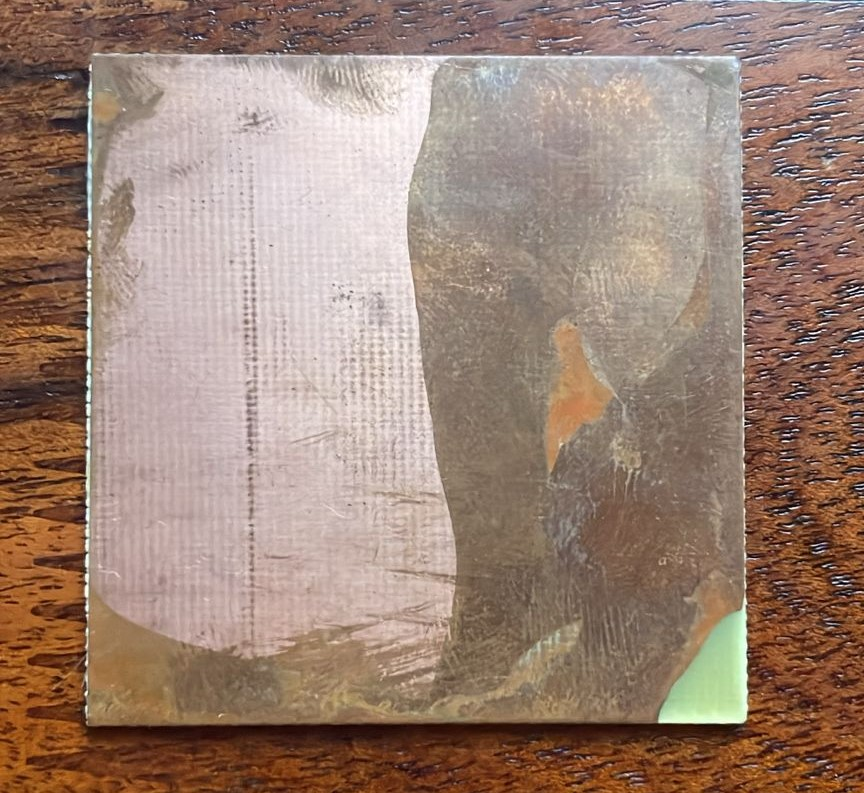
\includegraphics[width=0.4\textwidth]{Medición_h_y_t.jpeg}
    \caption{Medición de $\mathrm{h}$ y $\mathrm{t}$ de las placas.}
    \label{fig:Medición_h_y_t}
\end{figure}

Se observa en la \autoref{fig:Medición_h_y_t} que la esquina introducida al cloruro férrico, ya disuelto el cobre, permitió medir $\mathrm{h}$. Por otro lado, el resto de la placa tendrá un espesor de $\mathrm{h + 2t}$, donde el término $\mathrm{2t}$ surge del espesor de cobre a un lado y al otro del dieléctrico. 
    
Realizadas ambas mediciones con un micrómetro, se obtuvo el valor de ($\mathrm{h}$) y se dedujo el valor de ($\mathrm{t}$) como muestra la \autoref{eq:ht}:
    
\begin{equation}
    \begin{cases}
        \mathrm{h = 1.57 \ mm} \\
        \mathrm{t = 0.0275 \ mm}            
    \end{cases}
    \label{eq:ht}
\end{equation}
\\



\subsubsection{Medición de la permitividad eléctrica relativa $\mathrm{\epsilon_{r}}$} \label{section:sec_3.1.2}
Partiendo de los valores descritos en la \autoref{eq:ht}, se utilizaron las ecuaciones de la \autoref{section:sec_2.2} para diseñar microtiras que tengan una impedancia característica de $\mathrm{Z_{0} = 50 \ \Omega}$, asumiendo distintos valores de permitividad eléctrica relativa ($\mathrm{\epsilon_{r}}$). Nótese que la microtira que tenga un $\mathrm{\epsilon_{r}}$ más cercano al real de la placa, tendrá una mejor adaptación, la cual puede medirse con un roímetro. 
    
La \autoref{fig:Medición_e_r} muestra las 5 microtiras diseñadas para distintos valores de $\mathrm{\epsilon_{r}}$, entre las cuales varía su ancho para presentar la impedancia característica establecida. Tras realizar la medición con el roímetro, se dedujo que la microtira que presenta la mejor adaptación es la que presupuso que $\mathrm{\epsilon_{r} = 4}$, por lo que éste valor se tomó para realizar los cálculos posteriores que involucren este parámetro.

Para la realización de esta medición sobre la placa de prueba, fue necesario generar un layout con las dimensiones precisas de cada microtira, previamente calculada. Se utilizó el software KiCad versión 10.0 (Ver \autoref{fig:kicad}) y el método de transferencia de tóner, explicados a profundidad en la sección \autoref{section:sec_3.8.1}. 

\begin{figure}
    \centering
    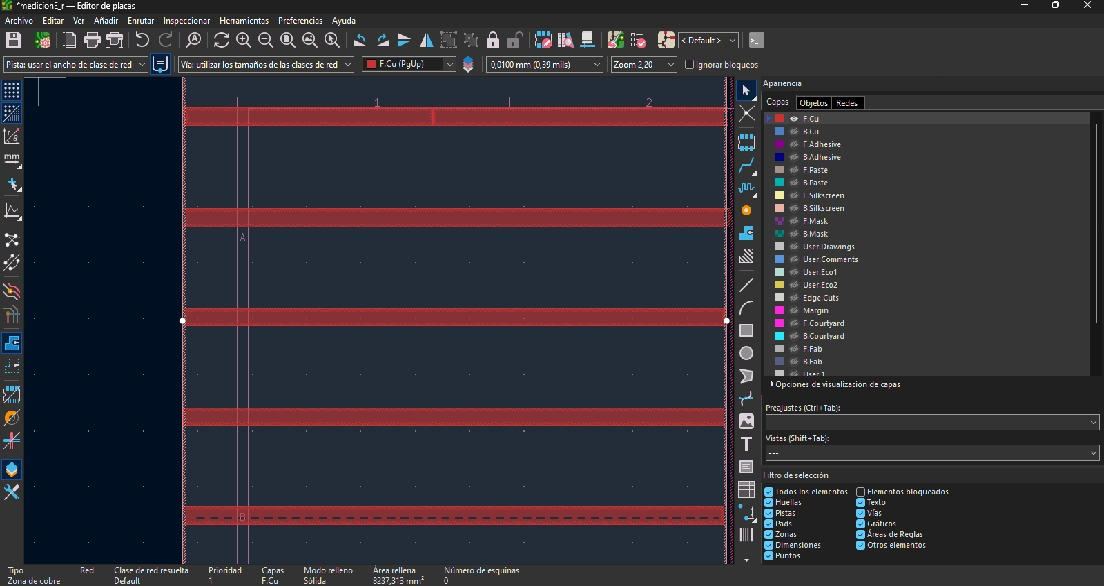
\includegraphics[width=0.85\linewidth]{Figuras/ki_cad.png}
    \caption{Entorno de trabajo con el layout a exportar.}
    \label{fig:kicad}
\end{figure}

\begin{figure}[!h]
    \centering
    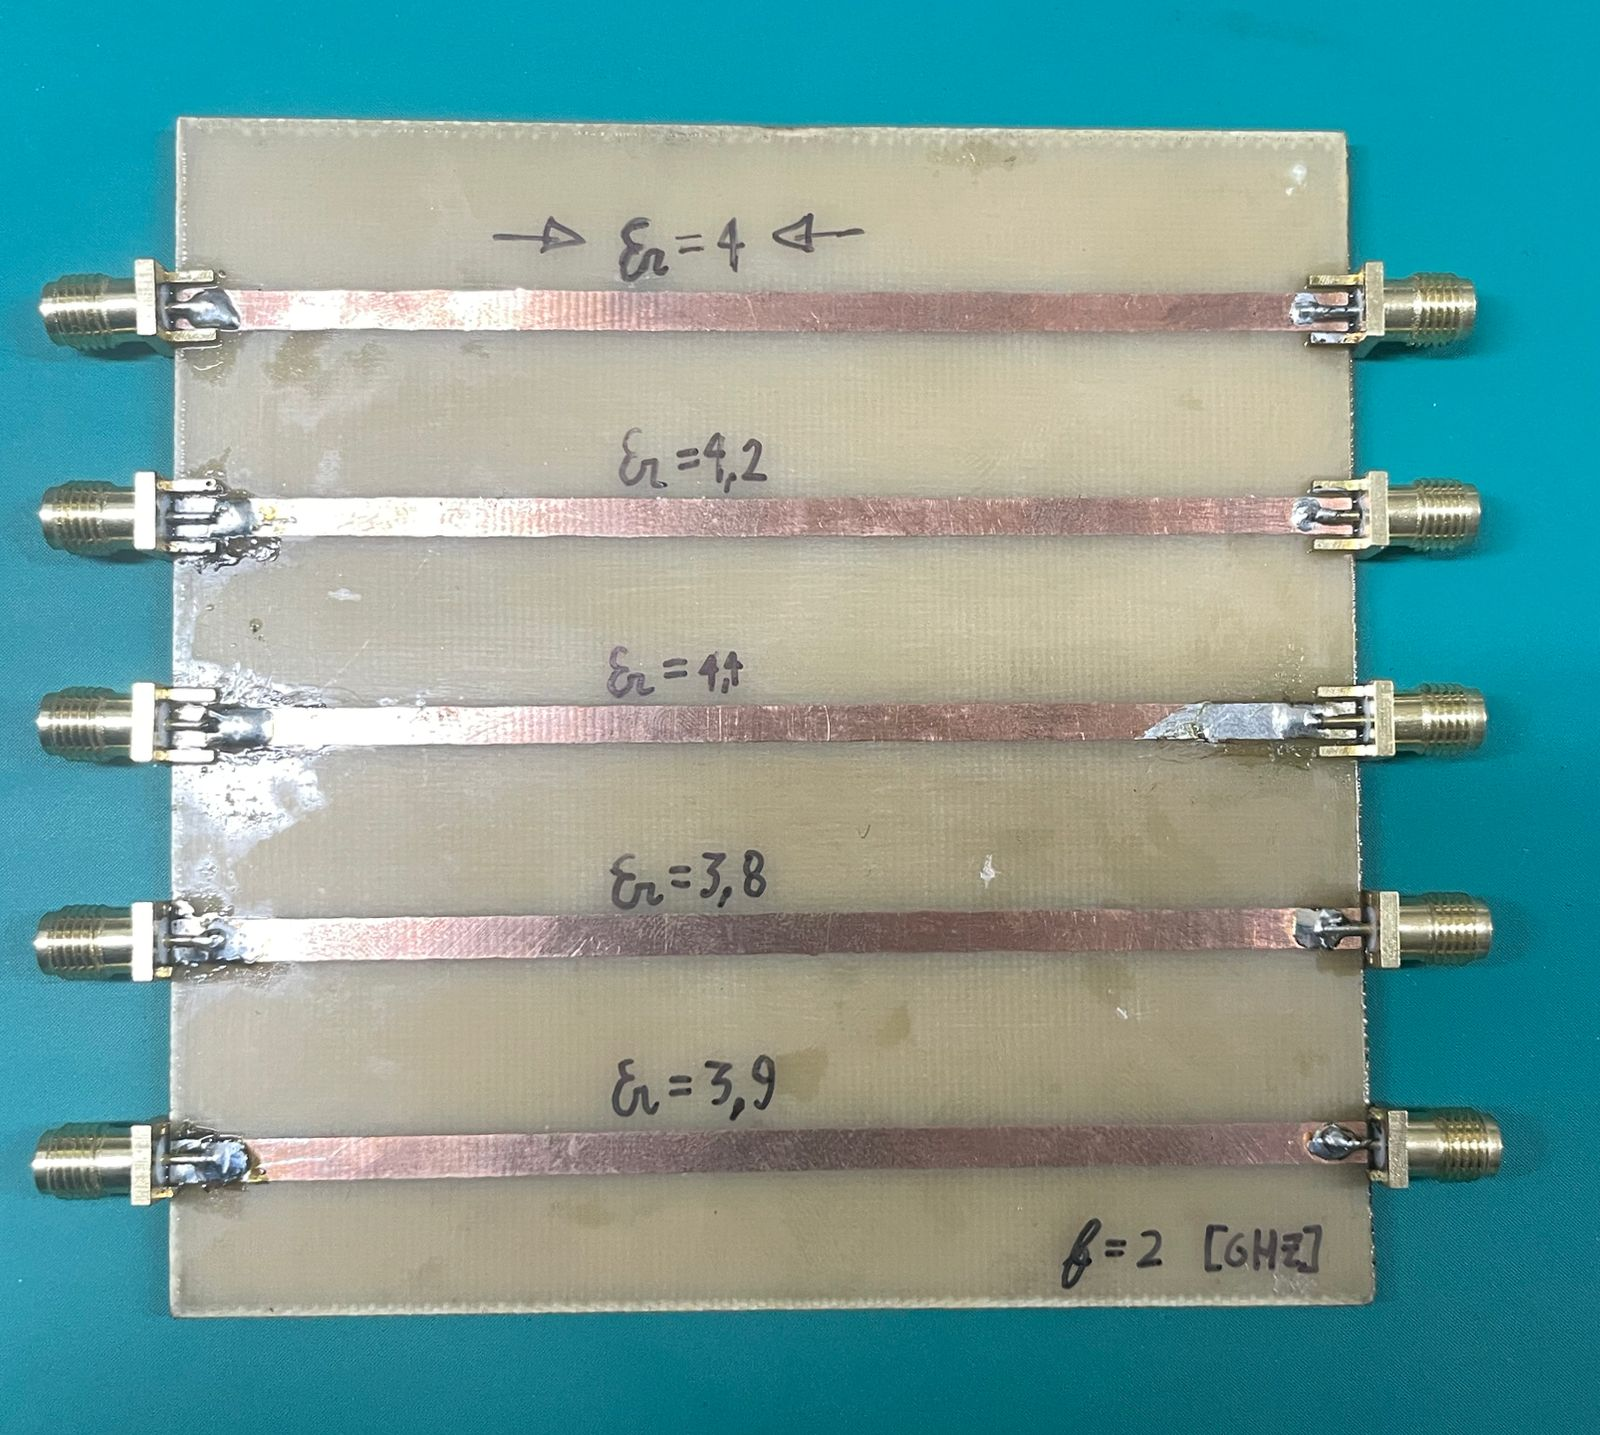
\includegraphics[width=0.7\textwidth]{Medición_e_r.jpeg}
    \caption{Medición de $\mathrm{\epsilon_{r}}$ de las placas.}
    \label{fig:Medición_e_r}
\end{figure}



\subsection{Selección de polarización} \label{section:sec_3.2}
El código de Python \cite{repo} barre los archivos de polarización de la librería de Infineon para el BJT BFP760 y realiza el análisis de estabilidad que describe la \autoref{section:sec_2.6}, lo que resultó en que todas las polarizaciones posibles presentan estabilidad condicional en $\mathrm{f = 2\ GHz}$.

Se decidió utilizar la polarización con $\mathrm{k}$ más cercano a 1, tal que la zona de operación estable cubra la mayor área en la Carta de Smith (Ver \autoref{eq:pol}). El análisis detallado del desarrollo de estabilidad se encuentra en la \autoref{section:sec_3.4}.
\begin{equation}
    \begin{cases}
        \mathrm{V_{CE} = 1 \ V} \\
        \mathrm{I_C = 40 \ mA}            
    \end{cases}
    \label{eq:pol}
\end{equation}



\subsection{Diseño de la Red de Polarización} \label{section:sec_3.3}
De acuerdo a los resultados deducidos en la \autoref{section:sec_3.2}, se procedió a diseñar una red de polarización que permita fijar la $\mathrm{I_{C}}$ del transistor para luego poder ajustar fácilmente $\mathrm{V_{CE}}$) sin modificar el primer valor, consiguiendo así polarizar de forma estable el BFP760.

Para ello se utilizó el simulador comercial y gratuito de electrónica LTspice y se incorporó el modelo del BFP760 a este entorno \cite{infineon_bfp760}. Luego se propusieron 2 formas de polarizar de forma precisa el transistor:

\begin{itemize}
    \item \underline{Método N°1: Polarización con Op-Amp}: Mediante el lazo de realimentación positiva del Op-Amp, se fija $\mathrm{I_{C}}$, con la posibilidad de ajustarla reemplazando $\mathrm{R_{sense}}$ por un potenciómetro, mientras que $\mathrm{V_{CE}}$ se ajusta también reemplazando $R_{2}$ por un potenciómetro, tal como muestra la \autoref{fig:Pol_Op-Amp}.
    \begin{figure}[!h]
        \centering
        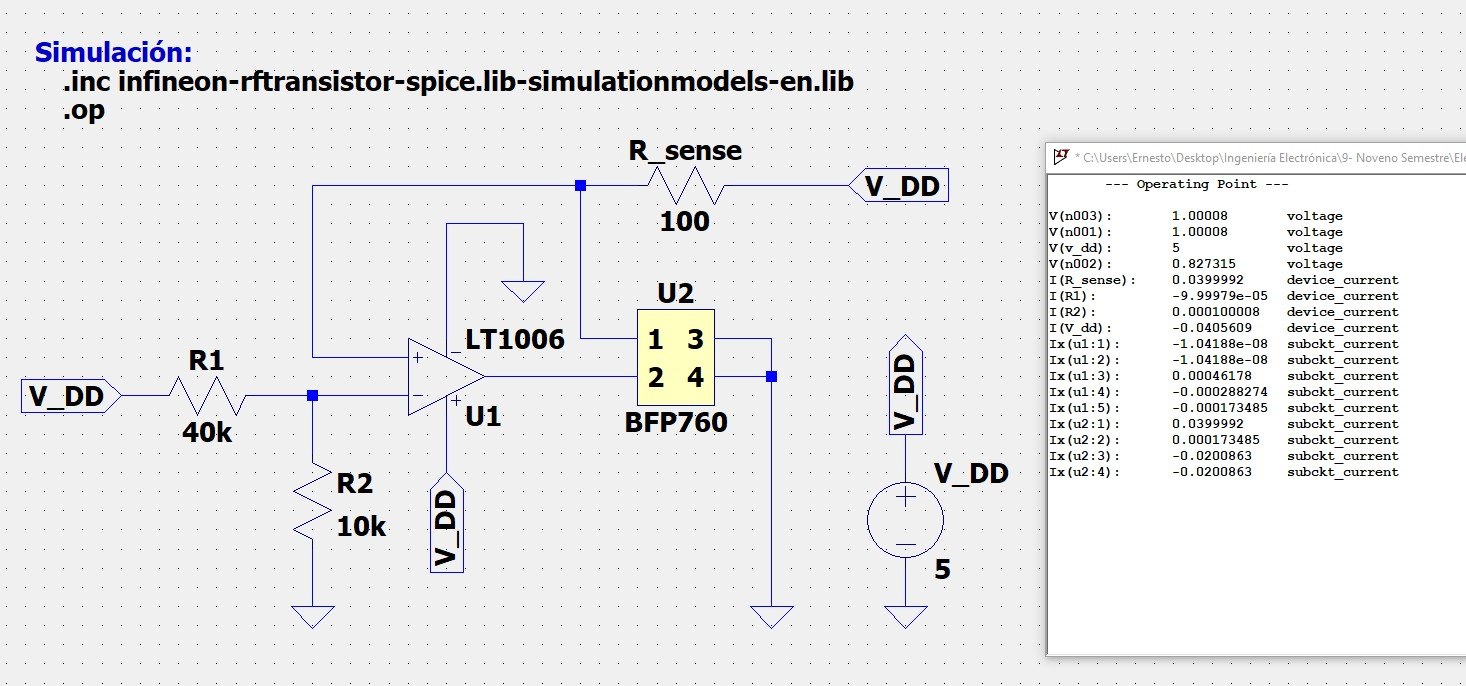
\includegraphics[width=0.9\textwidth]{Resultados con OPAMP.jpeg}
        \caption{Simulación de la Polarización con un Op-Amp.}
        \label{fig:Pol_Op-Amp}
    \end{figure}

    \item \underline{Método N°2: Polarización con LM317}: Este regulador presenta en su hoja de datos una configuración tal que opere como fuente de corriente \cite{ti_lm317}. Se coloca un potenciómetro en serie a $\mathrm{R_{B}}$ para el ajuste de $\mathrm{V_{CE}}$ y un potenciómetro en paralelo a $\mathrm{R_{set}}$ para ajustar $\mathrm{I_{C}}$ (Ver \autoref{fig:Pol_LM317}).
    \begin{figure}[!h]
        \centering
        
\includegraphics[width=0.9\textwidth]{Resultados con LM317.jpeg}
        \caption{Simulación de la Polarización con un LM317.}
        \label{fig:Pol_LM317}
    \end{figure}

\end{itemize}

Finalmente se decidió implementar la fuente de corriente con LM317, debido a su simpleza y versatilidad, ya que se puede configurar con cualquier regulador de tensión (no así el primer método es restrictivo en términos del Op-Amp a utilizar). La \autoref{fig:Pol_LM317_Fisica} muestra el circuito final en físico.
\begin{figure}[!h]
    \centering
    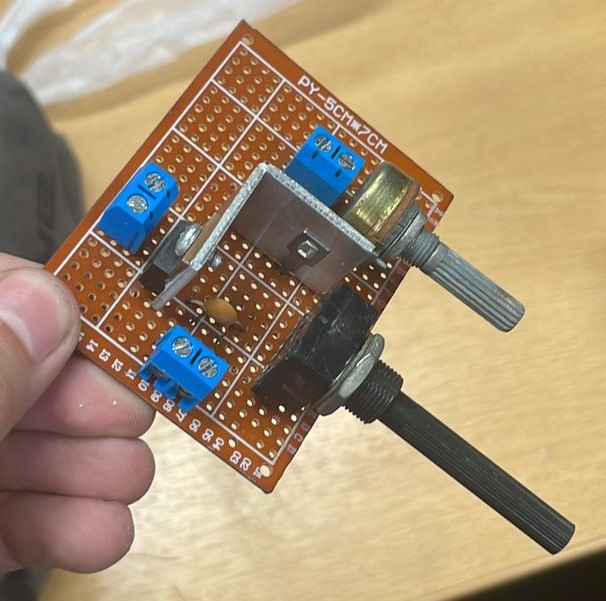
\includegraphics[width=0.5\textwidth]{Polarización_armada.jpeg}
    \caption{Imagen tomada del circuito armado en forma física.}
    \label{fig:Pol_LM317_Fisica}
\end{figure}



\subsection{Condiciones de Estabilidad} \label{section:sec_3.4}
Para el punto de polarización seleccionado en la \autoref{section:sec_3.2} en la frecuencia de diseño de $\mathrm{2 \ GHz}$, se extrajeron los parámetros de dispersión desde el archivo provisto por el fabricante. Los valores obtenidos, expresados en formato rectangular, son los siguientes:

\begin{equation}
    \mathrm{[S]} = 
    \begin{bmatrix} 
        \mathrm{-0.7091+j0.0895} & \mathrm{0.0346+j0.0218} \\ 
        \mathrm{2.5690+j8.9007} & \mathrm{-0.3168-j0.08429} 
    \end{bmatrix}
    \label{eq:S_params_values}
\end{equation}

A partir de la matriz de parámetros S, se evaluó analíticamente el criterio de Rollet mediante las ecuaciones descritas en la \autoref{section:sec_2.6}, obteniendo los siguientes resultados para el factor de estabilidad ($\mathrm{k}$) y el módulo del determinante ($\mathrm{|\Delta|}$):

\begin{equation}
    \begin{cases}
        \mathrm{k = 0.799868 } \\
        \mathrm{|\Delta| = 0.473693}
    \end{cases}
    \label{eq:k_delta_values}
\end{equation} 

Como se anticipó, al cumplirse que $\mathrm{k < 1}$ y $\mathrm{|\Delta| < 1}$, el dispositivo presenta estabilidad condicional. Por consiguiente, el uso de las ecuaciones de adaptación conjugada simultánea (\autoref{section:sec_2.7.1}) carece de validez matemática y física para este escenario. En su lugar, resulta mandatorio trazar los círculos de estabilidad en la Carta de Smith para seleccionar un punto de operación dentro de las regiones permitidas.

Bajo esta condición de estabilidad potencial, la figura de mérito que define la cota superior de ganancia alcanzable por el amplificador es la Ganancia Máxima Estable (MSG). Aplicando la \autoref{eq:MSG}, se determinó que la ganancia máxima teórica para este diseño es:

\begin{equation}
    \mathrm{MSG = 10 \cdot \log_{10} \left( \frac{|S_{21}|}{|S_{12}|} \right) = 23.550752 \ dB}
\end{equation}
\\



\subsection{Adaptación de Impedancias} \label{section:sec_3.5}
El procedimiento de adaptación consistió en el proceso detallado en \autoref{section:sec_2.7.2}, por lo que en primer lugar se graficó el círculo de estabilidad de salida y se realizó un barrido paramétrico discreto de posibles $\mathrm{\Gamma_L}$. Para cada valor ensayado, se calcularon los correspondientes $\mathrm{\Gamma_{in}}$, $\mathrm{\Gamma_{out}}$ y $\mathrm{\Gamma_S}$, y se graficó el círculo de estabilidad de entrada para verificar que los puntos $\mathrm{\Gamma_S}$ resultantes fuesen válidos (Ver \autoref{fig:Circulos_Estabilidad}).

El trazado de los círculos se realizó con el código de Python \cite{repo}, y se verificó con el programa Smith V4.1 para la polarización elegida y frecuencia dada, dando lugar a la \autoref{fig:smith}.

\begin{figure}[!h]
    \centering
    \fbox{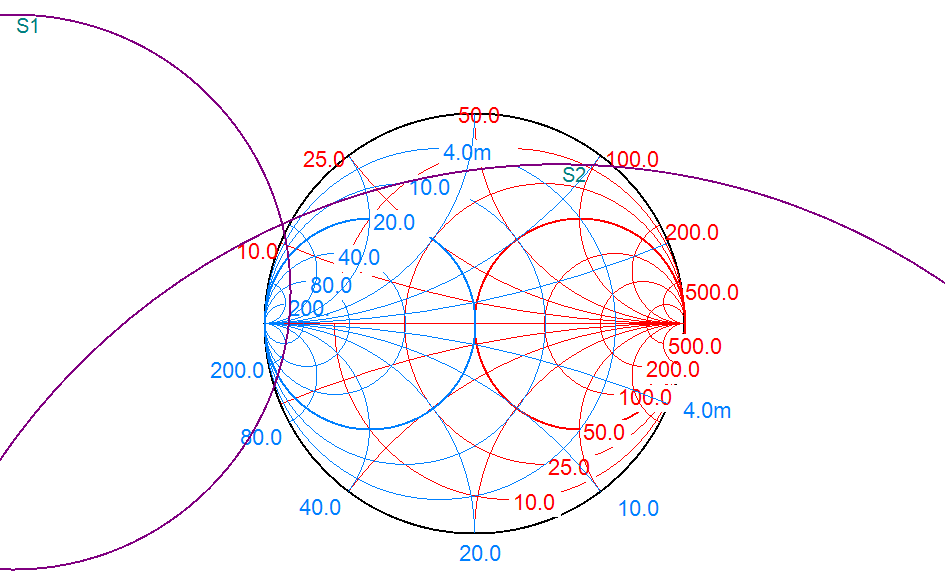
\includegraphics[width=0.8\linewidth]{Figuras/Smith2.png}}
    \caption{Círculos de estabilidad en la Carta de Smith.}
    \label{fig:smith}
\end{figure}

Se seleccionó un punto que no comprometa la estabilidad del sistema ante variaciones de la impedancia de carga o de la fuente, manteniéndose lejos de los límites de los círculos.
\begin{equation*}
    \mathrm{\Gamma_L = 0.95 \ \angle -45^\circ}
\end{equation*}

\begin{equation*}
    \mathrm{\Gamma_{in} = 0.6986 \ \angle \  149,86^\circ}
\end{equation*}

\begin{equation*}
    \mathrm{\Gamma_S = 0.6986 \  \angle -149,86^\circ}
\end{equation*}

\begin{equation*}
    \mathrm{\Gamma_{out} = 0.2909 \  \angle -68,94^\circ}
\end{equation*}

\begin{figure}[!h]
    \centering
    \fbox{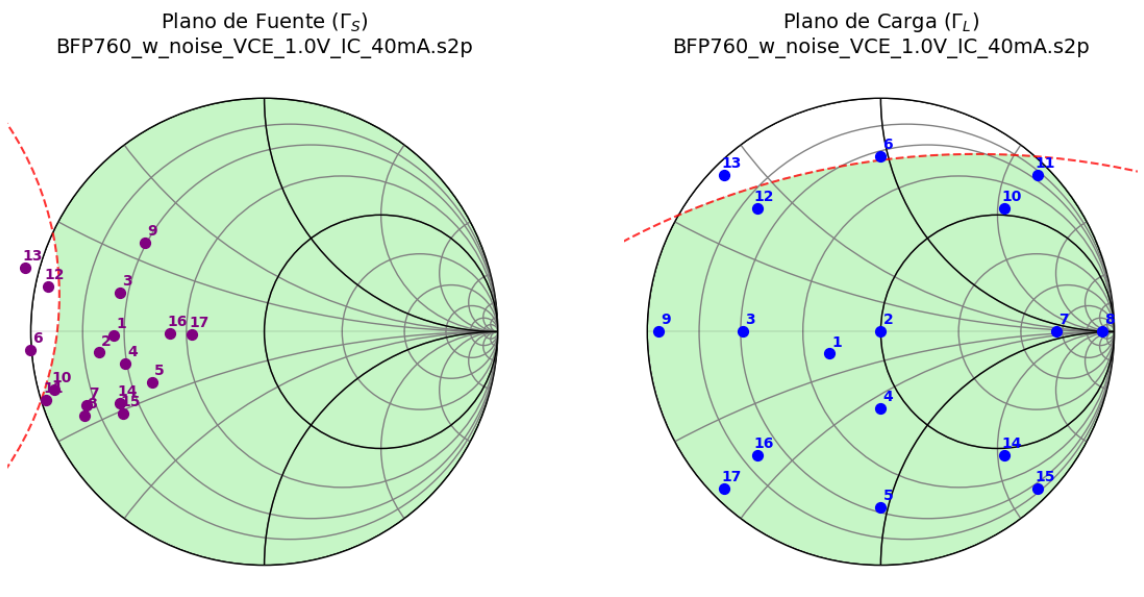
\includegraphics[width=1\linewidth]{Figuras/Smith.png}}
    \caption{Círculos de estabilidad y coeficientes de reflexión seleccionados en la Carta de Smith.}
    \label{fig:Circulos_Estabilidad}
\end{figure}

Finalmente, utilizando la \autoref{eq:Ztransistor}, se transformaron los coeficientes de reflexión $\mathrm{\Gamma_{in}}$ y $\mathrm{\Gamma_{out}}$ a sus correspondientes impedancias serie, considerando $\mathrm{Z_0 = 50 \ \Omega}$:
\begin{equation}
    \begin{cases}
        \mathrm{Z_{in(s)} = 9.4942 + j13.0076 \ \Omega} \\
        \mathrm{Z_{out(s)} = 52.2718 -j31.0033 \ \Omega}
    \end{cases}
    \label{eq:Z_serie_calculadas}
\end{equation}

Dado que la red de adaptación en la entrada es de carácter inductivo y la de salida capacitivo, se implementaron topologías de adaptación específicas para cada puerto, las cuales se detallan a continuación.
\\



\subsubsection{Adaptación a la entrada}
Al presentar el transistor una impedancia de entrada con componente reactiva inductiva, se optó por una topología de adaptación basada en un transformador de $\lambda/4$ y un stub en circuito abierto conectado en paralelo, encargado de sintetizar la capacitancia necesaria para cancelar la susceptancia inductiva del puerto (Ver \autoref{fig:Adapt_in}).

Para esto se debió transformar al modelo paralelo la impedancia de entrada utilizando la \autoref{eq:serie_a_paralelo}, e igualando la reactancia capacitiva del stub a la parte imaginaria de $\mathrm{Z_{in(p)}}$, se determinó el valor del capacitor de adaptación ($\mathrm{C_{in}}$). Simultáneamente, la adaptación de la componente puramente resistiva hacia la impedancia del sistema ($50 \ \Omega$) se logró calculando la impedancia característica del transformador ($\mathrm{Z_{0(in)}}$) mediante la \autoref{eq:Z_m_calc}. Ver los resultados en la \autoref{eq:adapt_in} y la \autoref{eq:Z_0in}.

\begin{equation}
    \mathrm{Z_{in(p)} = 27.3154 \parallel j19.9373 \ \Omega}
    \label{eq:Z_paralelo_calculadas}
\end{equation}

\begin{equation}
    \mathrm{C_{in} = 3.99138 \ pF}
    \label{eq:adapt_in}
\end{equation}

\begin{equation}
    \mathrm{Z_{0(in)} = 36.9563 \ \Omega}
    \label{eq:Z_0in}
\end{equation}

\begin{figure}[!h]
    \centering
    \fbox{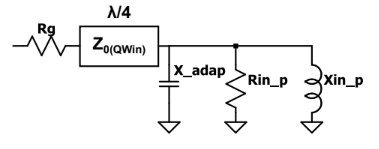
\includegraphics[width=0.55\linewidth]{Figuras/Adapt_in.png}}
    \caption{Red de adaptación a la entrada.}
    \label{fig:Adapt_in}
\end{figure}



\subsubsection{Adaptación a la salida}
Para el puerto de salida, cuya impedancia intrínseca presenta un comportamiento capacitivo, se procedió de forma análoga (Ver \autoref{fig:Adapt_out}). Mediante la inclusión de un transformador de $\lambda/4$, se adaptó la resistencia equivalente de salida a los $50 \ \Omega$ del sistema, determinando su impedancia característica $\mathrm{Z_{0(out)}}$.

La componente reactiva se compensó mediante un segundo stub en circuito abierto encargado de sintetizar el capacitor ($\mathrm{C_{out}}$). Se ven los resultados en la \autoref{eq:adapt_out} y la \autoref{eq:Z_0out}.
\begin{equation}
    \mathrm{C_{out} = 0.944 \ pF}
    \label{eq:adapt_out}
\end{equation}

\begin{equation}
    \mathrm{Z_{0(out)} = 51.1233 \ \Omega}
    \label{eq:Z_0out}
\end{equation}

\begin{figure}[!h]
    \centering
    \fbox{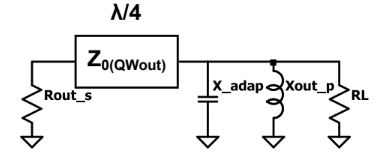
\includegraphics[width=0.45\linewidth]{Figuras/Adapt_out.png}}
    \caption{Red de adaptación a la salida.}
    \label{fig:Adapt_out}
\end{figure}



\subsection{Síntesis de Microtiras} \label{section:sec_3.6}
Con los valores analíticos de las redes de adaptación definidos en la \autoref{section:sec_3.5} y de las redes de polarización de la \autoref{section:sec_3.3}, se procedió a realizar la síntesis geométrica de las microtiras. Para esto se aplicaron las ecuaciones de Hammerstad (Ver \autoref{section:sec_2.2}) en el código de Python \cite{repo} contemplando los parámetros físicos del sustrato medidos en la \autoref{section:sec_3.1}. 

Se calculó la permitividad efectiva ($\mathrm{\epsilon_{eff}}$) y se dimensionaron los anchos efectivos ($\mathrm{W_{eff}}$) y las longitudes físicas ($\mathrm{d}$) de cada tramo del circuito.
\\



\subsubsection{Líneas de adaptación} \label{section:sec_3.6.1}
Para los transformadores de $\lambda/4$ y las líneas principales de conducción de la señal de RF, se obtuvieron las siguientes dimensiones físicas:

\begin{table}[!h]
    \centering
    \renewcommand{\arraystretch}{1.2}
    \begin{tabular}{|c|c|c|c|c|} \hline
        \textbf{Elemento} & $\mathbf{Z_c \ [\Omega]}$ & $\mathbf{\epsilon_{eff}}$ & $\mathbf{W_{eff} \ [mm]}$ & $\mathbf{d \ [mm]}$ \\ \hline
        Líneas principales & 50.00 & 3.0733 & 3.2736 & - \\ \hline
        Transformador Entrada & 36.95 & 3.1933 & 5.1694 & 20.9849 \\ \hline
        Transformador Salida & 51.12 & 3.0642 & 3.1561 & 21.4222 \\ \hline
    \end{tabular}
    \caption{Dimensiones geométricas de las líneas principales y transformadores.}
    \label{tab:dims_lineas}
\end{table}



\subsubsection{Elementos reactivos (Stubs)} \label{section:sec_3.6.2}
Las longitudes eléctricas necesarias para sintetizar los capacitores de adaptación $\mathrm{C_{in}}$ y $\mathrm{C_{out}}$ mediante \textit{stubs} en circuito abierto con impedancia característica de $50 \ \Omega$, arrojaron los siguientes resultados geométricos:
\begin{table}[!h]
    \centering
    \renewcommand{\arraystretch}{1.2}
    \begin{tabular}{|c|c|c|c|} \hline
        \textbf{Elemento} & $\mathbf{Capacitancia \ [pF]}$ & $\mathbf{W_{eff} \ [mm]}$ & $\mathbf{d \ [mm]}$ \\ \hline
        Stub de Entrada & 3.9914 & 3.2736 & 16.2238 \\ \hline
        Stub de Salida & 0.94397 & 3.2736 & 7.2902 \\ \hline
    \end{tabular}
    \caption{Dimensiones geométricas de los stubs de adaptación.}
    \label{tab:dims_stubs}
\end{table}



\subsubsection{Red de polarización en alta frecuencia} \label{section:sec_3.6.3}
El diseño del choque de RF constó de lo detallado en la \autoref{section:sec_2.9}. Los resultados para la red de polarización resultaron en:
\begin{table}[!h]
    \centering
    \renewcommand{\arraystretch}{1.2}
    \begin{tabular}{|c|c|c|c|} \hline
        \textbf{Elemento} & $\mathbf{Impedancia\ caracteristica\ [\Omega]}$ & $\mathbf{W_{eff} \ [mm]}$ & $\mathbf{d \ [mm]}$ \\ \hline
        Inductor de choque & 100 &  0.8277 & 22.3551 \\ \hline
        Capacitor de desacople & 40 & 4.6106 & 21.0881 \\ \hline
    \end{tabular}
    \caption{Dimensiones geométricas de los elementos de la red de polarización.}
    \label{tab:dims_pol}
\end{table}



\subsection{Simulaciones en ADS} \label{section:sec_3.7}
A fin de validar los cálculos analíticos y la síntesis geométrica desarrollados previamente, se modeló el circuito en el entorno de simulación Advanced Design System (ADS). El objetivo de esta etapa fue verificar el comportamiento de los parámetros S en la frecuencia de trabajo según lo diseñado analíticamente.
\\



\subsubsection{Simulación del diseño ideal adaptado} \label{section:sec_3.7.1}
En primera instancia, se ensambló el esquemático de simulación incorporando el modelo del transistor BFP760 junto con los elementos de adaptación sintetizados en la \autoref{section:sec_3.6}. Para modelar las microtiras, se utilizaron los componentes paramétricos de línea (\texttt{MLIN}) y circuitos abiertos (\texttt{MLOC}).
 \begin{figure}[!h]
     \centering
     \fbox{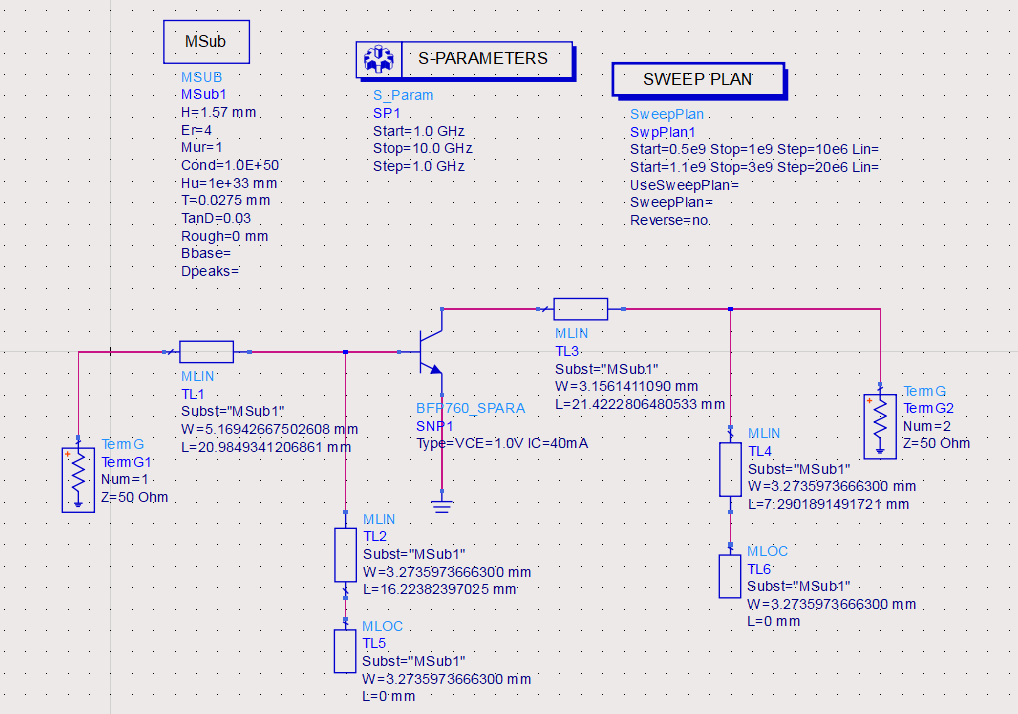
\includegraphics[width=0.85\linewidth]{Figuras/ADS_Ideal_Schematic.png}}
     \caption{Esquemático de la red de adaptación ideal en ADS.}
     \label{fig:ADS_Ideal_Schem}
 \end{figure}

Al correr una simulación de parámetros S en un barrido de frecuencias centrado en $2 \ \mathrm{GHz}$, se obtuvieron los resultados mostrados en la \autoref{fig:ADS_Ideal_Graph}. 

Se observa que a la frecuencia de diseño, ($\mathrm{S_{21}}$) presenta un valor cercano a la MSG teórica estimada, sin embargo puede notarse que mientras que las pérdidas de retorno de entrada ($\mathrm{S_{11}}$) tienen un valor elevado, no así las de salida ($\mathrm{S_{22}}$). Este resultado fue esperable porque ya que no era posible aplicar la adaptación conjugada simultánea, por lo que uno de los puertos no estará adaptado.
 \begin{figure}[!h]
     \centering
     \fbox{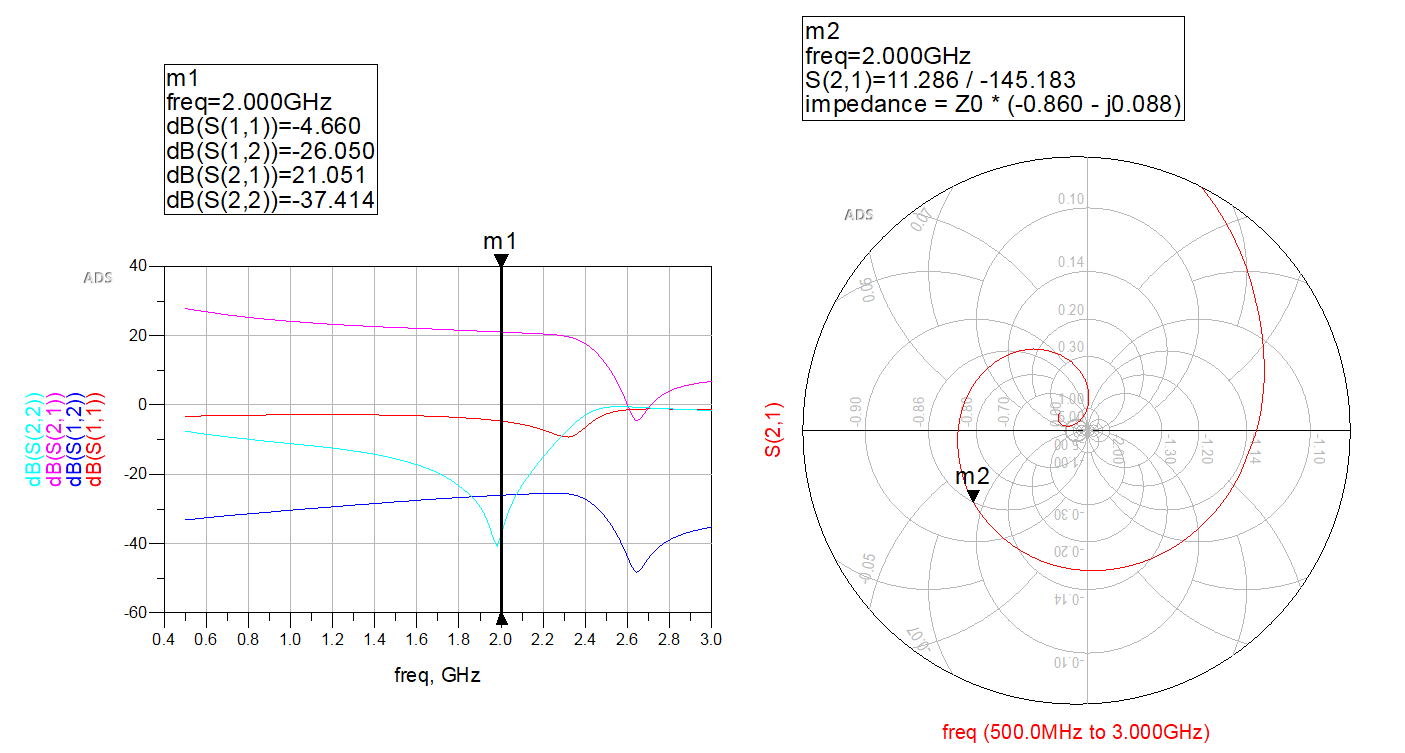
\includegraphics[width=0.85\linewidth]{Figuras/ADS_Ideal_Graph.png}}
     \caption{Parámetros S resultantes de la simulación de adaptación ideal.}
     \label{fig:ADS_Ideal_Graph}
 \end{figure}



\subsubsection{Incorporación de tapers y líneas principales} \label{section:sec_3.7.2}
Se introdujeron tapers para mitigar el efecto explicado en la \autoref{section:sec_2.10}, modelados mediante el componente \texttt{MTAPER} de ADS. Debido a que el taper posee una longitud física y altera la fase de la onda, se utilizó el código de Python \cite{repo} para recalcular la longitud de las líneas correspondientes y compensar este tramo adicional. Se definieron tapers de $3 \ \mathrm{mm}$ de longitud y los valores finales se detallan en la \autoref{tab:dims_pol_tapers}.
\begin{table}[!h]
    \centering
    \renewcommand{\arraystretch}{1.2}
    \begin{tabular}{|c|c|c|c|}
        \hline
        \textbf{Elemento compensado} & $\mathbf{d \ original \ [mm]}$ & $\mathbf{\Delta d_{taper} \ [mm]}$ & $\mathbf{d_{final} \ [mm]}$ \\ \hline
        Inductor de choque & 22.3550 & -1.8121 & 20.5429 \\ \hline
        Capacitor desacople & 21.0880 & -0.3253 & 20.7627 \\ \hline
        Capacitor de entrada & 16.2238 & -0.4582 & 15.7656 \\ \hline
        Capacitor de salida & 7.2902 & -0.4582 & 6.8320 \\ \hline
    \end{tabular}
    \caption{Longitudes compensadas de la red de polarización tras incluir Tapers de $3 \ \mathrm{mm}$.}
    \label{tab:dims_pol_tapers}
\end{table}

También se añaden a la simulación las líneas principales de 50 $\Omega$, los ``GAPS'' en los stubs para corregir capacitancias al momento de la implementación física, y los capacitores cerámicos que aíslan los instrumentos del laboratorio de la continua de polarización del circuito (Ver \autoref{fig:ADS_Fisico_Schem}). Se ejecutó una simulación considerando el circuito completo. Las gráficas definitivas evidenciaron un gran deterioro en los coeficientes de reflexión de ambos puertos, y una baja considerable de ganancia comparada a ($\mathrm{S_{21}}$).
\begin{figure}[!h]
    \centering
    \fbox{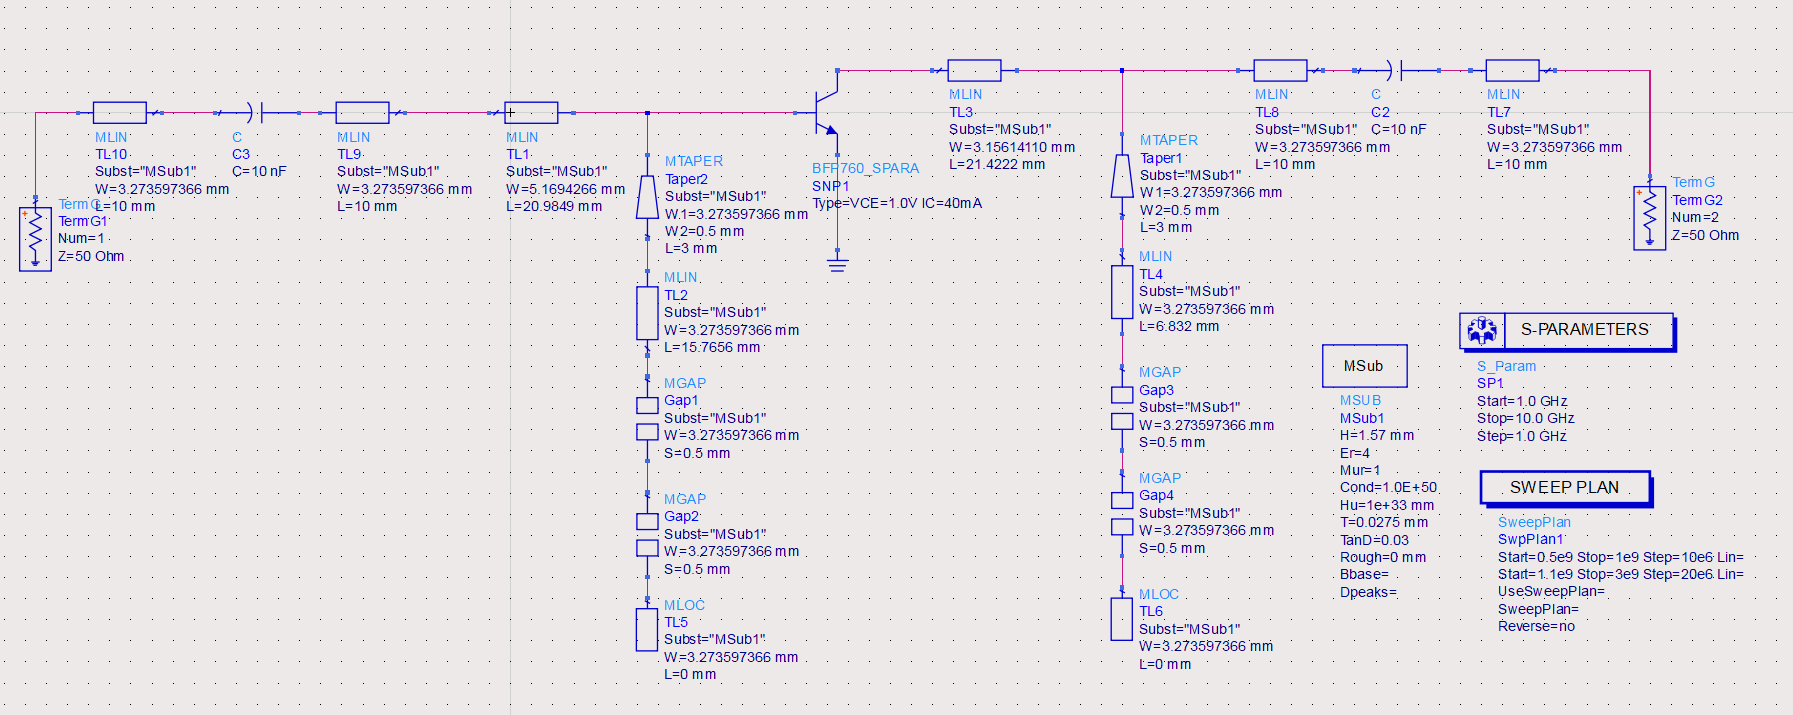
\includegraphics[width=1\linewidth]{Figuras/ADS_Fisico_Schematic.png}}
    \caption{Esquemático físico completo en ADS.}
    \label{fig:ADS_Fisico_Schem}
\end{figure}

\begin{figure}[!h]
    \centering
    \fbox{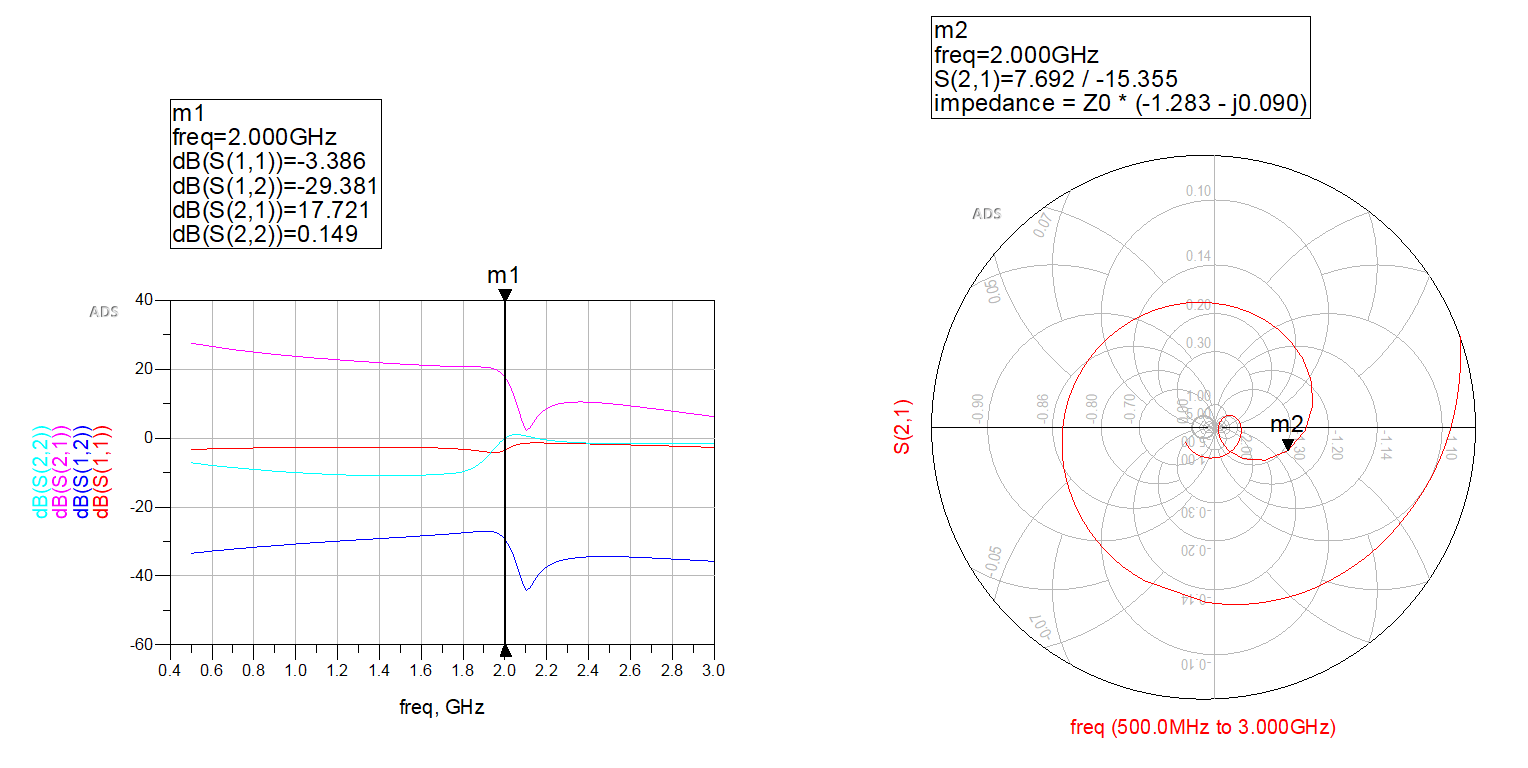
\includegraphics[width=0.85\linewidth]{Figuras/ADS_Fisico_Graph.png}}
    \caption{Parámetros S del modelo físico simulado.}
    \label{fig:ADS_Fisico_Graph}
\end{figure}



\subsubsection{Ajuste fino de componentes}\label{section:sec_3.7.3}
Ante la degradación de la respuesta frecuencial producida por los elementos parásitos, se recurrió a la herramienta de optimización manual ``Tuning'' de ADS. El objetivo de este procedimiento fue realizar un ajuste fino de las dimensiones de los transformadores de $\lambda/4$ y de las longitudes de los stubs de adaptación para evaluar dinámicamente cambios en la respuesta en la frecuencia de operación de $2 \ \mathrm{GHz}$.

Tras sintonizar analíticamente los parámetros mencionados, se obtuvieron las curvas de respuesta expuestas en la \autoref{fig:ADS_Tuning_Graph}. Se observa una notable recuperación de la ganancia ($\mathrm{S_{21}}$) en comparación con el escenario degradado. Adicionalmente, mientras que la adaptación de entrada mantuvo un comportamiento controlado, el coeficiente de reflexión de salida ($\mathrm{S_{22}}$) logró optimizarse hasta alcanzar niveles significativamente menores que los del modelo ideal preliminar.
 \begin{figure}[!h]
     \centering
      \fbox{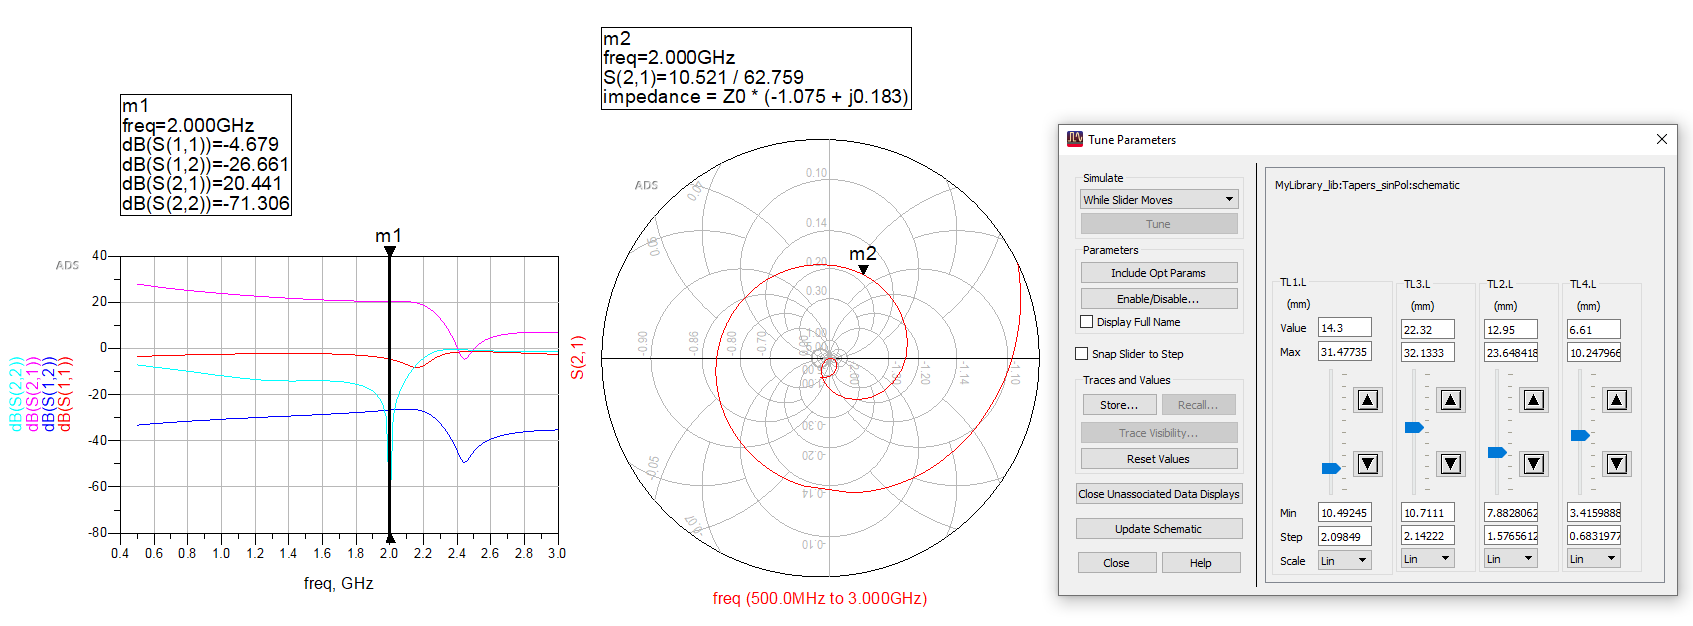
\includegraphics[width=1\linewidth]{Figuras/ADS_Tuning_Graph.png}}
     \caption{Parámetros S del modelo físico con ajuste fino.}
     \label{fig:ADS_Tuning_Graph}
 \end{figure}

 
\subsection{Armado Físico del Circuito} \label{section:sec_3.8}
Una vez validado el diseño mediante simulaciones, se procedió a la materialización del amplificador. Para esto se requiere de: 
\begin{itemize}
    \item Placa de cobre FR4.
    \item Conectores SMA 1.6 mm.
    \item Transistor BFP760.
    \item Elementos del circuito de polarización
\end{itemize}

Para llegar a un circuito físico final, se dividió el proceso en dos etapas:

\begin{itemize}
\item \underline{Layout}: Consta de la conexión de los elementos que conforman el circuito esquemático y que culmina con el diseño final (en formato Gerber o plano .svg).
\item \underline{Fabricación}: Se toma el diseño final para la placa de cobre y se utilizan métodos de transferencia hasta tener un circuito listo para conectarse y medir.
\end{itemize}


\subsubsection{Diseño del Layout del circuito:}

Se presentaron 2 alternativas posibles de entornos de trabajo para utilizar:

\begin{itemize}
    
    \item \textbf{KiCad 10.0.0}: Herramienta de diseño de placas con varias ``layers'' y soporte para generar esquemáticos (con parámetros concentrados), plasmar las rutas de interconexión y posteriormente un layout.
    
    \item \textbf{Inkscape}: Herramienta de dibujo tipo Canvas, que permite introducir formas geométricas con dimensiones y ubicaciones precisas, que mantienen su tamaño en el archivo exportable, lo cual se traduce a superficies de cobre igualmente precisas.
    
\end{itemize}

El entorno de trabajo elegido fue Inkscape, debido a la precisión del tamaño del archivo a exportar, además de las facilidades que ofrece para la edición y ubicación de las figuras para las microtiras, con un flujo de trabajo más intuitivo al trabajar en una sola capa y no multilayer, como es el caso de KiCad.

Las pautas para la conformación del archivo .svg final fueron: 

 \begin{itemize}
    \item \underline{Diseño espejado}: Se realizó el diseño de layout espejado horizontalmente, ya que llegado el momento de imprimir las pistas, quedan orientadas como se muestra en la simulación, ya que de no hacerlo, la disposición invertida de los terminales del transistor habría impedido su correcto montaje y acoplamiento con las microtiras.
    
    \item \underline{Conexión de emisor a masa}: Se colocaron superficies o islas de cobre en los dos terminales de emisor del transistor, para posteriormente perforar las mismas y hacer la conexión a masa (Ver \autoref{section:sec_3.8.3}).
    
    \item \underline{Longitud de las líneas principales}: Las microtiras de 50 $\Omega$ deben aumentar su longitud para abarcar el largo entre los lados de la placa (10 cm), y así extenderse hasta los conectores SMA.

    \item \underline{Separación entre terminales metálicos del transistor}: Para soldar correctamente los terminales del BFP760, es necesario hacer una precisa separación entre ellos. Para eso se utilizó el diagrama del exténsil del componente que se muestra en \autoref{fig:ext.png}, ubicado en el datasheet del BJT BFP760 \cite{infineon_bfp760}.

\end{itemize}

     \begin{figure}[!h]
     \centering
      \fbox{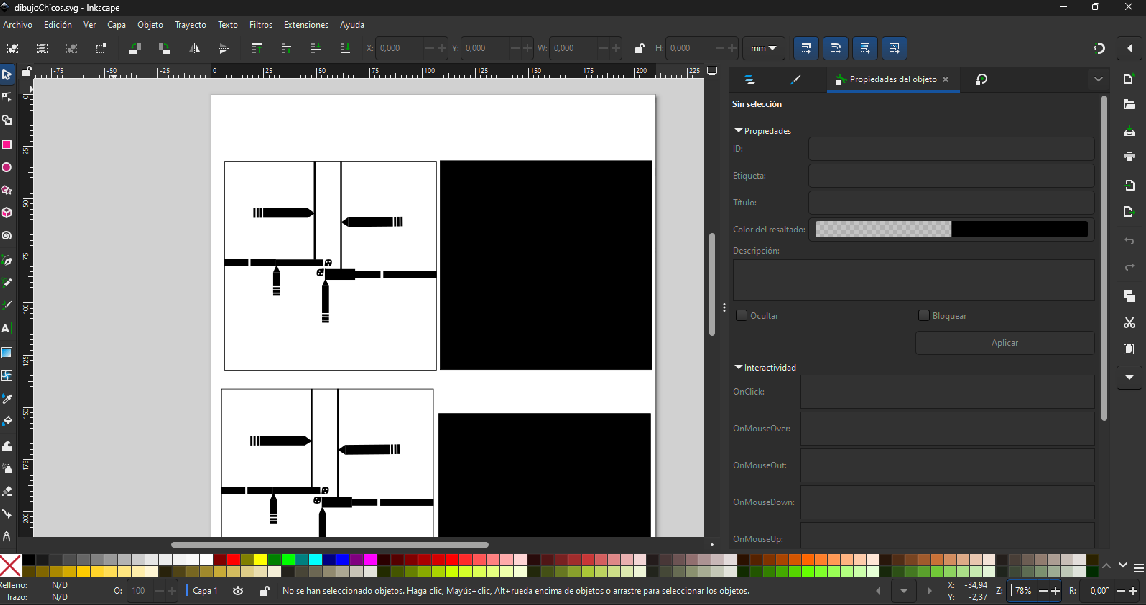
\includegraphics[width=1\linewidth]{Figuras/entorno_ink.png}}
     \caption{Entorno de trabajo Inkscape con el circuito final a imprimir.}
     \label{fig:entorno_ink}
 \end{figure}

    \begin{figure}[!h]
     \centering
      \fbox{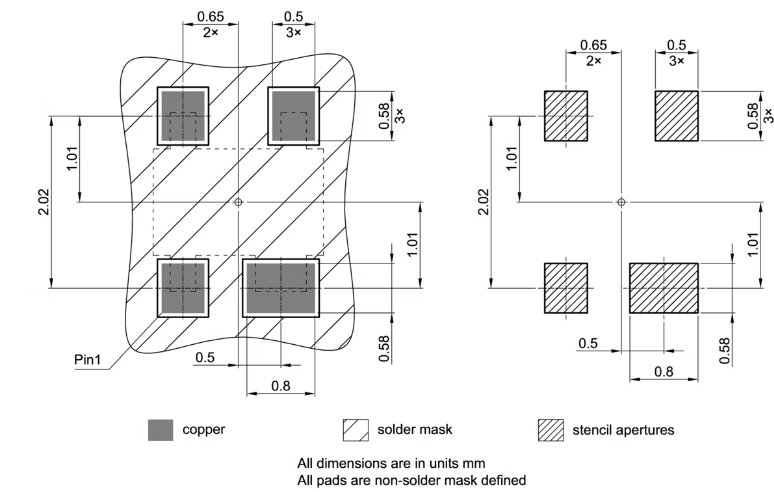
\includegraphics[width=0.8\linewidth]{Figuras/ext.png}}
     \caption{Huella para el montaje del empaquetado- PG-SOT343-4-1.}
     \label{fig:ext.png}
 \end{figure}
 
    \begin{figure}[!h]
     \centering
      \fbox{
\includegraphics[width=0.35\linewidth]{Figuras/ext_ki.png}}
     \caption{Espaciado en el layout.}
     \label{fig:ext_ki.png}
 \end{figure}




\subsubsection{Fabricación de la placa de circuito impreso (PCB)}\label{section:sec_3.8.2}
El diseño del layout final se exportó y se transfirió a la placa de sustrato FR4 virgen, previamente caracterizada en la \autoref{section:sec_3.1}. 

Para plasmar las pistas de cobre, se empleó el método de transferencia térmica de tóner (conocido comúnmente como método de planchado), que consta de la impresión en papel satinado o de revista del circuito utilizando una impresora láser, con los trazos de tinta en los espacios donde se desea que el cobre permanezca. Luego, habiendo retirado impurezas y óxido en el cobre a utilizar, se aplicó presión y calor uniforme para fijar el tóner sobre la placa.

Posteriormente, se sumergió el sustrato en cloruro férrico con el objetivo de disolver el cobre expuesto que no se encontraba enmascarado con el tóner. Al finalizar la disolución, las pistas diseñadas quedaron establecidas. 

Para concluir, se realizó una remoción de los restos de tóner remanentes con alcohol isopropílico, garantizando una superficie de cobre limpia y apta para el proceso de soldadura.
\\



\subsubsection{Tratamiento del plano de masa y vías}\label{section:sec_3.8.3}
Dado que la topología de microtiras requiere un plano de masa continuo en la cara inferior, se perforó el sustrato FR4 utilizando un mini-torno de alta velocidad (tipo Dremel), habilitando perforaciones en islas de cobre específicas, para los emisores del transistor. 

La conexión eléctrica entre estas islas de la cara superior y el plano sólido inferior se materializó insertando conductores metálicos (obtenidos a partir de terminales de resistencias recicladas). Estos conductores fueron soldados al ras en ambas caras de la placa para asegurar una óptima continuidad eléctrica y minimizar las inductancias parásitas asociadas a la longitud de la vía.
\\



\subsubsection{Soldadura de componentes e integración del sistema completo}
En primer lugar, se soldó el transistor BJT BFP760. Debido a su alta sensibilidad a estrés térmico, se empleó un soldador de punta fina y flux, apuntando a uniones metálicas brillantes, precisas y sin excesos de estaño que pudieran alterar el comportamiento del modelo.

A continuación, se posicionaron los capacitores cerámicos de bloqueo de continua, y por último, se montaron los conectores SMA de $50 \ \Omega$ en los bordes de la placa para los puertos de entrada y salida, asegurando una transición mecánica y eléctrica robusta desde el pin central hacia la pista correspondiente.

Finalmente, la placa de RF se interconectó con la etapa de polarización en continua (basada en el regulador LM317, detallada en la \autoref{section:sec_3.3}). La alimentación de corriente continua ($\mathrm{V_{CE}}$ e $\mathrm{I_C}$) se inyectó a través de los nodos previstos en los inductores de choque.
\\



\subsection{Mediciones y resultados} \label{section:sec_3.9}
Concluido el ensamblaje del prototipo físico, se procedió a la etapa de medición en el laboratorio. Esta fase se dividió en dos instancias: la verificación estática del punto de trabajo en corriente continua y la medición de la respuesta en frecuencia.
\\



\subsubsection{Verificación del punto de polarización}
Antes de inyectar señales de radiofrecuencia, se corroboró el correcto funcionamiento de la red de polarización activa. Alimentando el circuito con una fuente de tensión de $5\ \text{V}$, se ajustaron los potenciómetros de la fuente de corriente diseñada hasta alcanzar los valores de reposo deseados para el BJT BFP760 ($\mathrm{V_{CE}} = 1\ \text{V}$ y $\mathrm{I_C} = 40\ \text{mA}$).
\\



\subsubsection{Caracterización de las pérdidas del instrumental}
Previo a evaluar la ganancia del circuito, resultó indispensable cuantificar la atenuación introducida por el cableado utilizado en el conexionado, con el fin de compensar este valor al momento de analizar la respuesta neta del amplificador. 

En la \autoref{fig:perdida_pot} se observa que, ante una potencia de inyección de $-30\ \text{dBm}$ desde el generador, el nivel de potencia recibido en el analizador a la frecuencia de diseño de $2\ \text{GHz}$ fue de $-37.4\ \text{dBm}$. Por consiguiente, se determinó una pérdida de inserción en los cables de $7.4\ \text{dB}$.

Las mediciones se realizaron con estos cables durante todo el proceso restante.

\begin{figure}[!h]
    \centering
    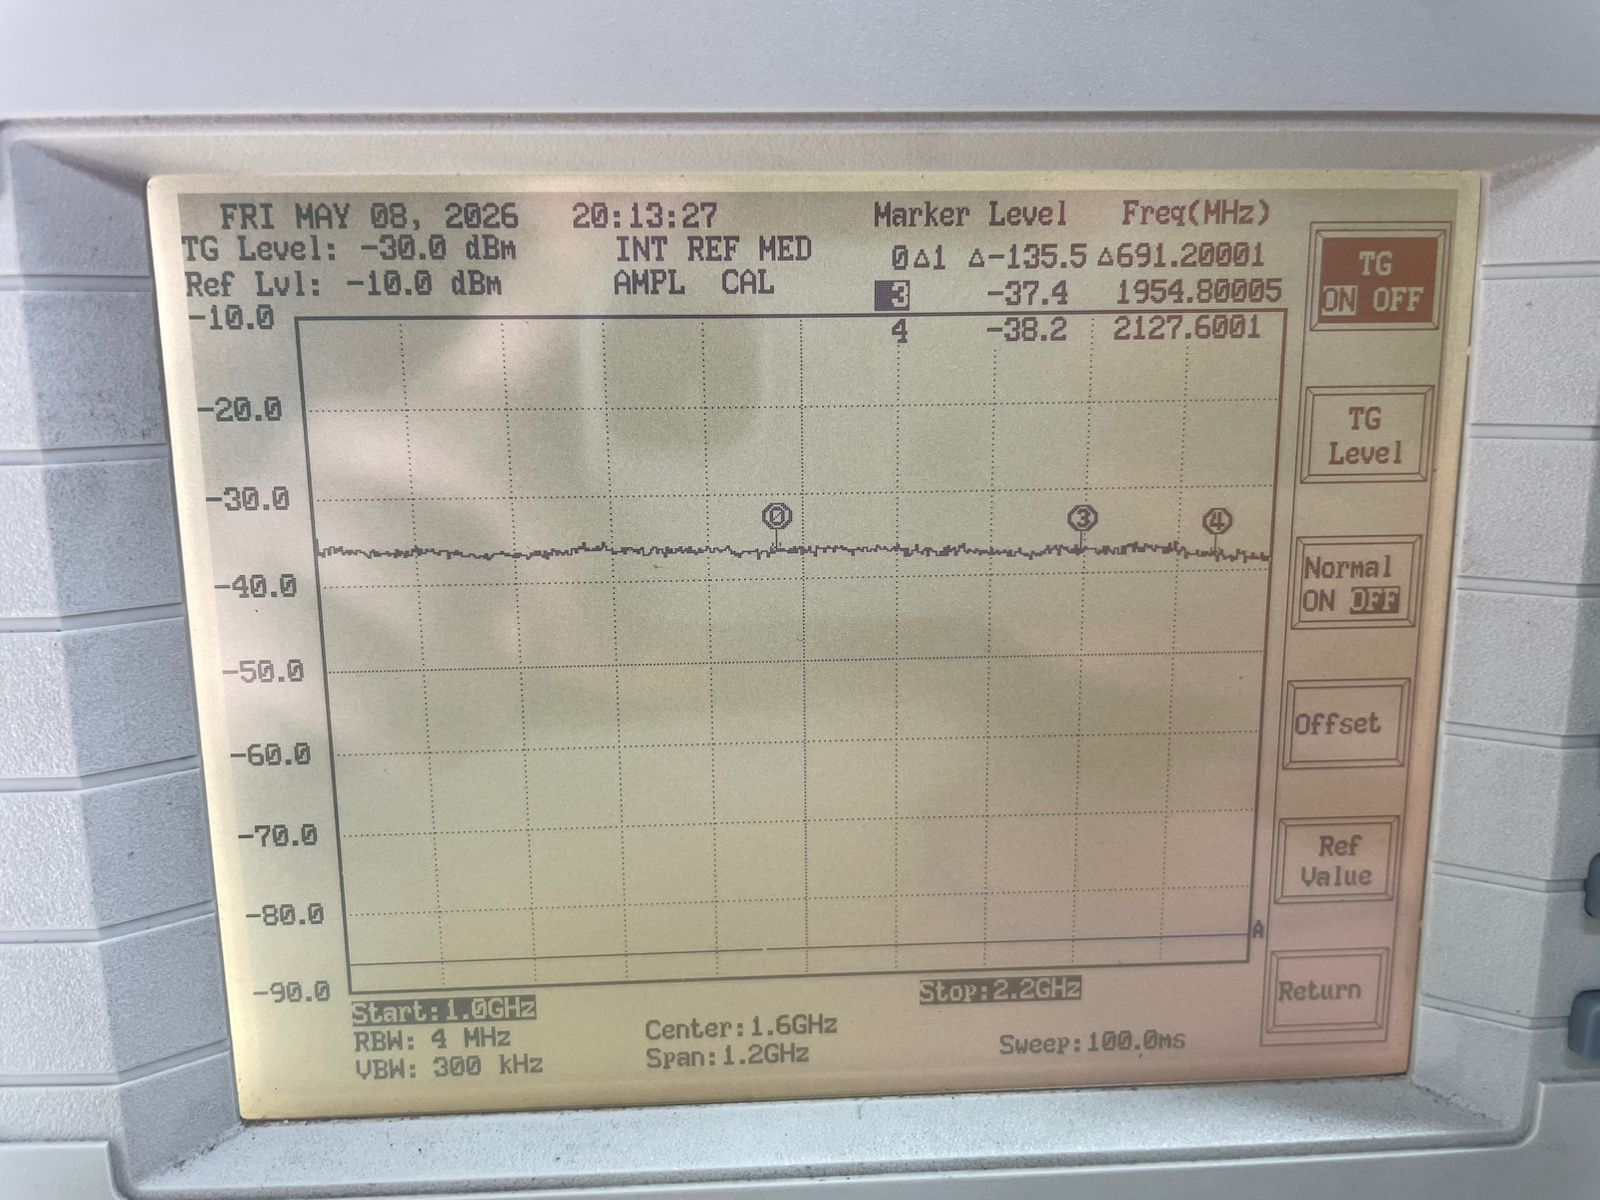
\includegraphics[width=0.7\linewidth]{Figuras/perdida_pot.png}
    \caption{Medición de la pérdida de potencia en los cables de interconexión a $2\ \text{GHz}$.}
    \label{fig:perdida_pot}
\end{figure}
\\



\subsubsection{Primera medición}

Tras conectar el prototipo al analizador de espectro, se inyectó una señal a un nivel de potencia de $-30\ \text{dBm}$, garantizando así una operación en el régimen de pequeña señal. 

La respuesta inicial del circuito, expuesta en la \autoref{fig:osc}, evidenció un claro comportamiento oscilatorio y fuertemente inestable. Adicionalmente, a la frecuencia de interés ($2\ \text{GHz}$), se registró un nivel de salida de $-52.2\ \text{dBm}$, lo que se traduce en una severa atenuación de $22.2\ \text{dB}$ respecto a la potencia inyectada (sin descontar las pérdidas del cable), demostrando una completa desadaptación de la red.
\\

\begin{figure}[!h]
    \centering
    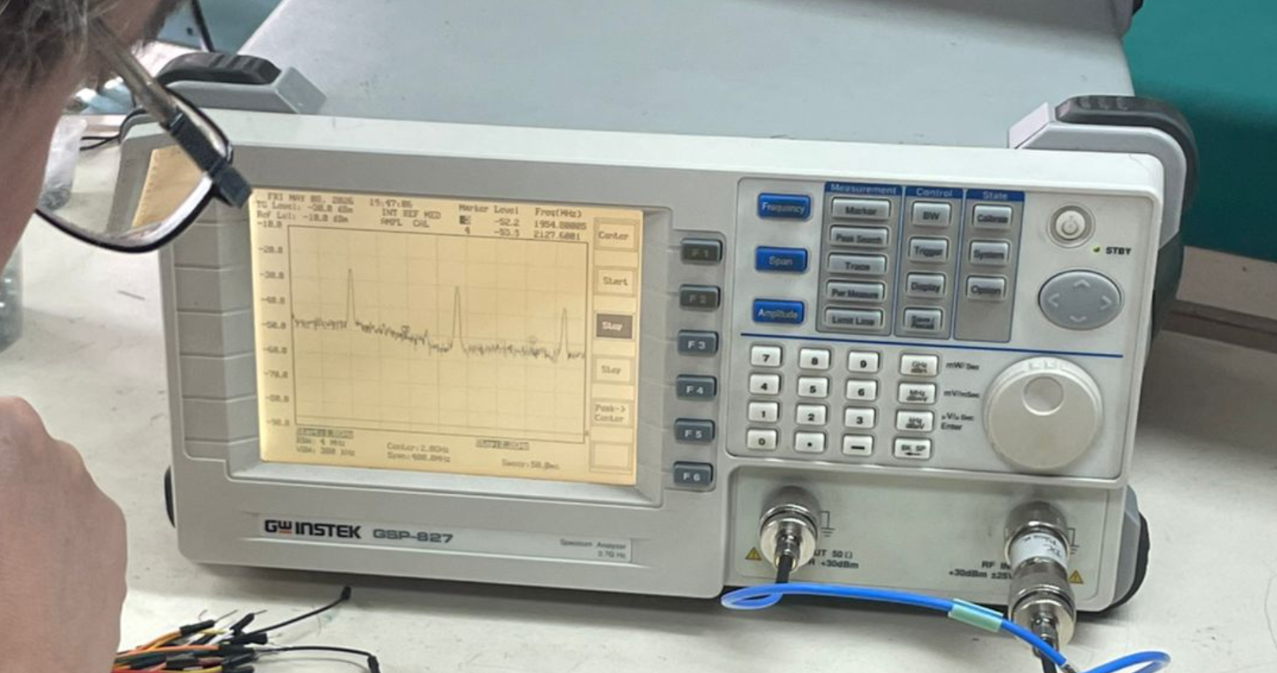
\includegraphics[width=0.8\linewidth]{osc.png}
    \caption{Respuesta inicial del prototipo exhibiendo comportamiento oscilatorio.}
    \label{fig:osc}
\end{figure}
\\



\subsubsection{Ajuste y optimización del circuito}
Ante la presencia de inestabilidades, se llevaron a cabo una serie de modificaciones empíricas para identificar y mitigar la causa de la oscilación.

En una primera instancia, se sospechó de resonancias en la red de polarización. Para descartar este efecto, se interrumpió físicamente la continuidad de las microtiras correspondientes a los inductores de choque y capacitores de desacople, reemplazándolas por componentes discretos. No obstante, la oscilación persistió y no se observó una mejora significativa en la ganancia.

Posteriormente, se recurrió al uso de los ``gaps'' incorporados en el layout original. Se observó que, al reducir la capacitancia de la red de adaptación de salida, la respuesta experimentaba un ligero incremento de ganancia, aunque sin lograr el cese de la oscilación. En consecuencia, se procedió a intervenir la red de adaptación de entrada: al aumentar el valor de la capacitancia de adaptación en dicho puerto, el circuito modificó drásticamente su comportamiento, logrando estabilizar el sistema (extinción de la oscilación) y elevando la potencia de salida a $-29.1\ \text{dBm}$ a $2\ \text{GHz}$. Se adjunta una imagen de la versión final del circuito armado en físico en \autoref{fig:final}.

\begin{figure}[!h]
    \centering
    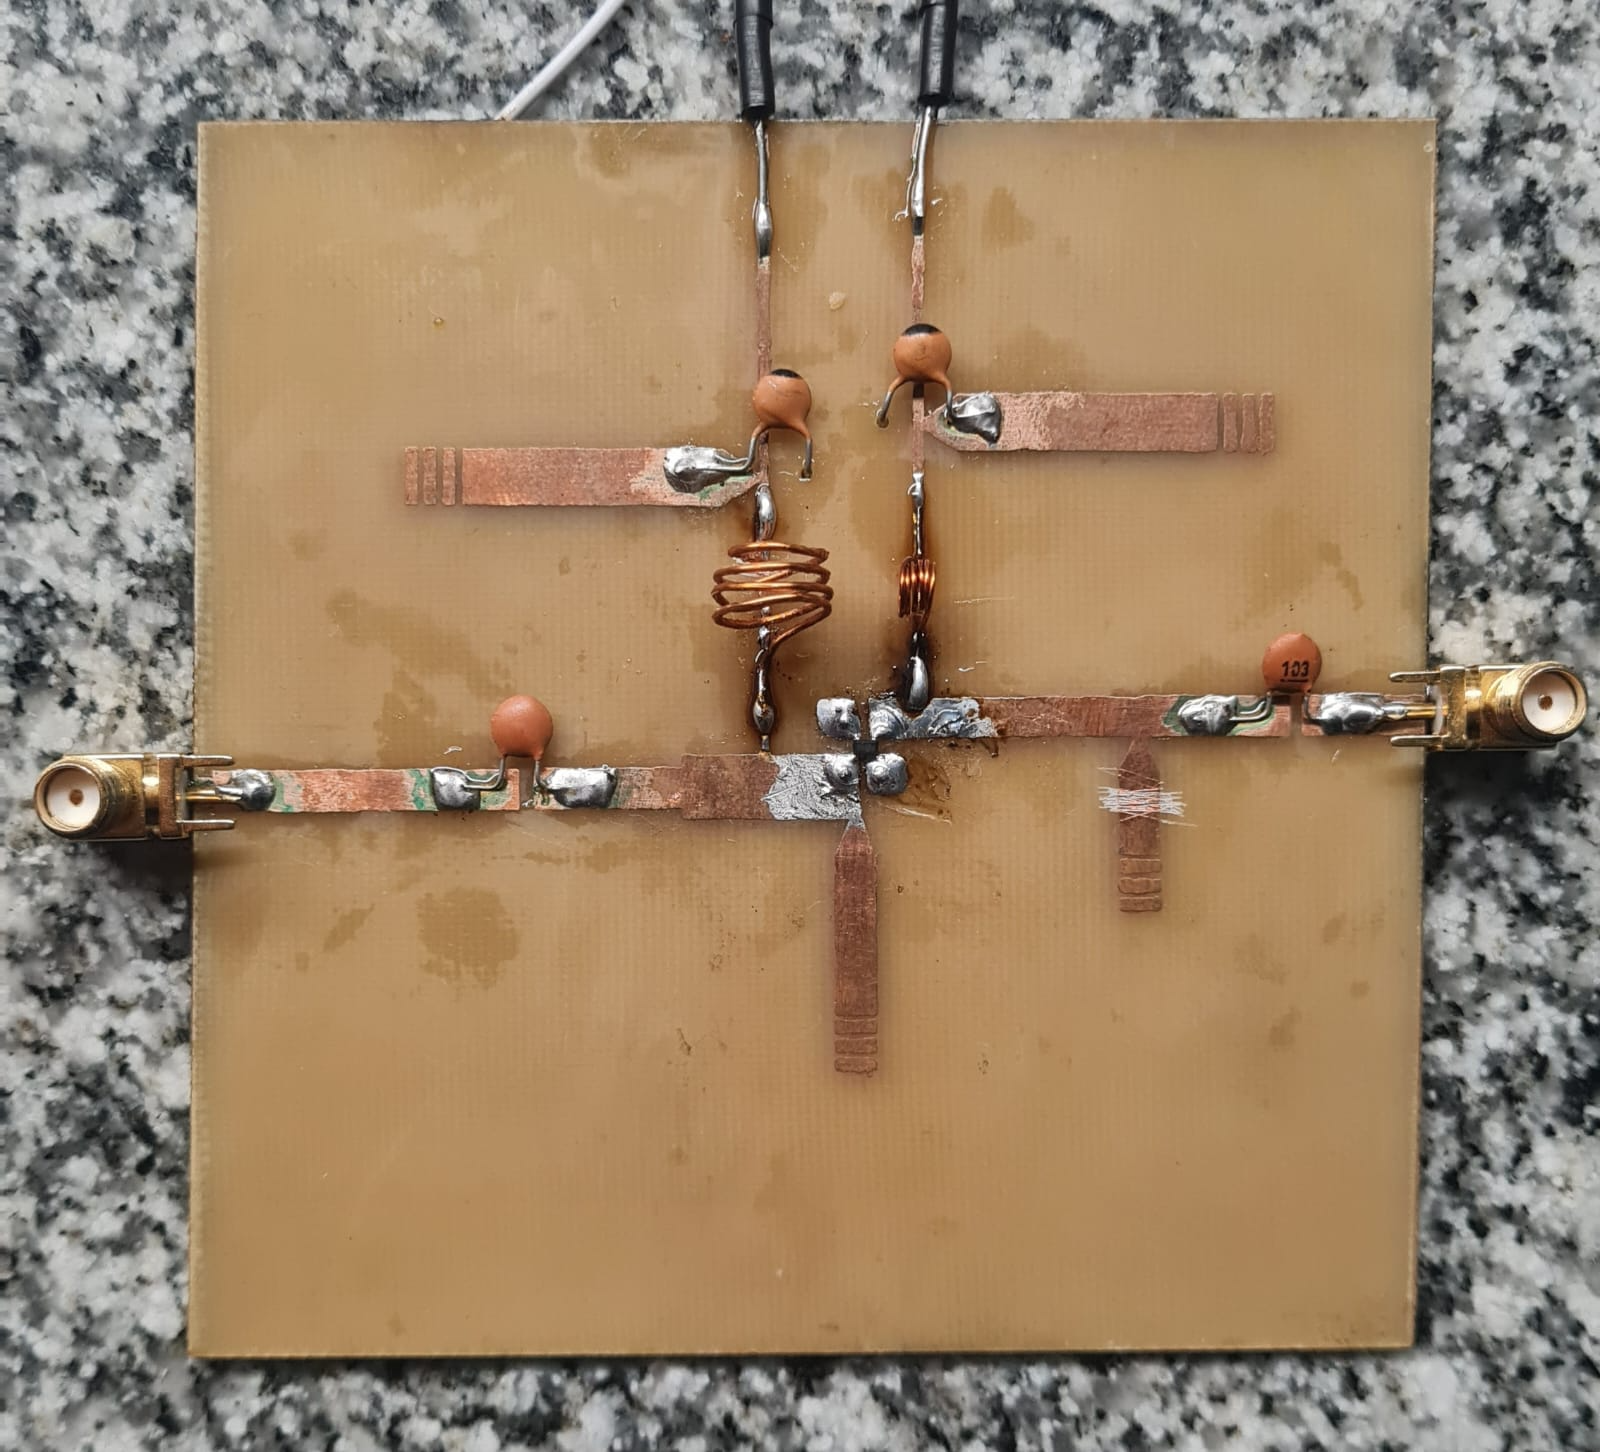
\includegraphics[width=0.7\linewidth]{Figuras/final.png}
    \caption{Versión final del circuito físico.}
    \label{fig:final}
\end{figure}

La respuesta final del circuito estabilizado se expone en la \autoref{fig:gain}. Para determinar la ganancia neta del amplificador, es necesario calcular la diferencia entre la potencia leída a la salida y la potencia inyectada, compensando las atenuaciones introducidas por los cables de interconexión (medidas previamente en $7.4 \ \mathrm{dB}$). El resultado, detallado en la \autoref{eq:gain}, arroja una ganancia final de $8.3 \ \mathrm{dB}$.

\begin{equation}
    G = P_{\mathrm{out}} - P_{\mathrm{in}} + L_{\mathrm{cables}} = -29.1 \ \mathrm{dBm} - (-30.0 \ \mathrm{dBm}) + 7.4 \ \mathrm{dB} = 8.3 \ \mathrm{dB}
    \label{eq:gain}
\end{equation}



\begin{figure}[!h]
    \centering
    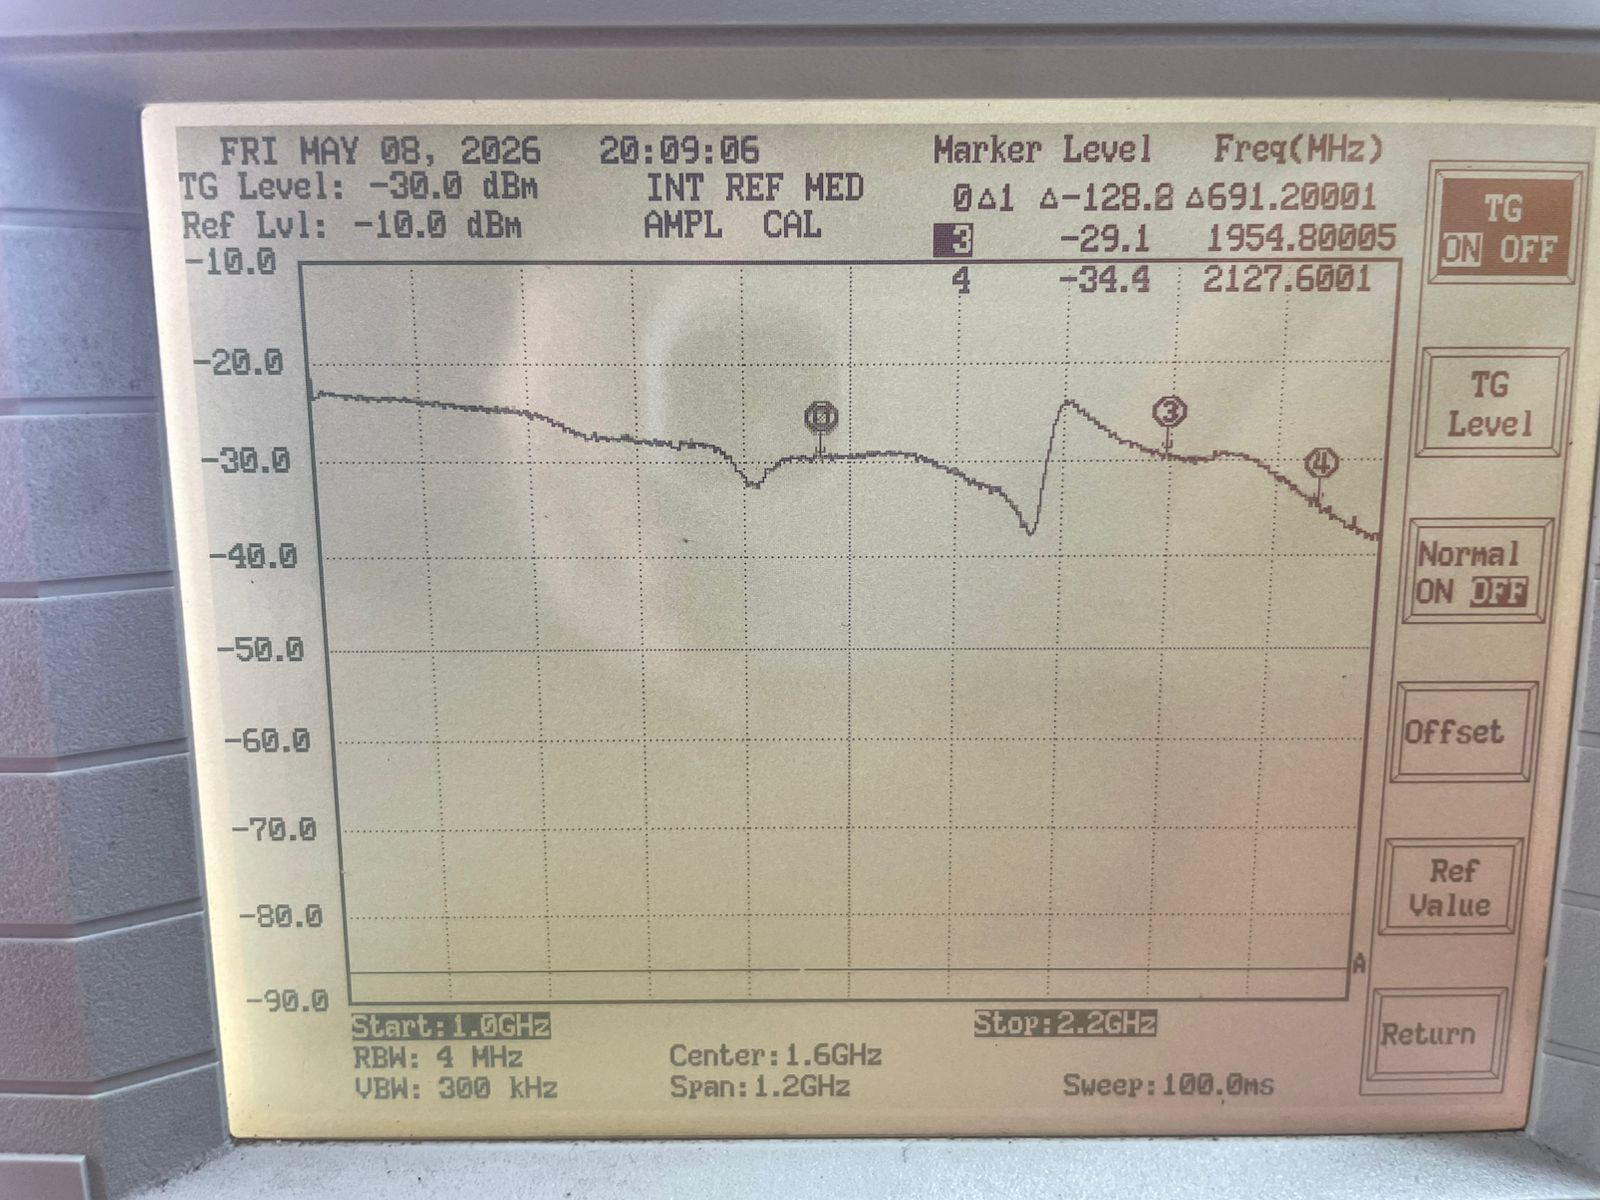
\includegraphics[width=0.7\linewidth]{Figuras/Gain.png}
    \caption{Respuesta en frecuencia estabilizada tras el ajuste empírico de las redes de adaptación.}
    \label{fig:gain}
\end{figure}




\newpage

\section{Conclusiones} \label{section:sec_4}

El desarrollo del presente trabajo transitó el flujo completo de diseño de un amplificador de radiofrecuencia a $2 \ \mathrm{GHz}$, abarcando desde la síntesis analítica y simulación, hasta la implementación del prototipo físico. 

Durante la etapa de validación práctica, se evidenciaron los desafíos en microondas. La primera evaluación del circuito arrojó un comportamiento oscilatorio severo, producto de desadaptaciones e imperfecciones en el circuito no contemplados por el modelo lineal ideal que fue simulado. No obstante, mediante una etapa de ajuste manual sobre las redes de adaptación, se logró extinguir la oscilación y estabilizar el sistema ajustando la capacitancia de entrada. 

Como resultado definitivo, el amplificador demostró ser funcional, entregando una ganancia neta real de $8.3 \ \mathrm{dB}$ a la frecuencia de diseño. La \autoref{tab:comparativa_final} resume los valores de mérito obtenidos en las distintas etapas del proyecto.

\begin{table}[!h]
    \centering
    \renewcommand{\arraystretch}{1.3}
    \begin{tabular}{|c|c|}
    \hline
    \textbf{Etapa del diseño} & \textbf{Ganancia ($\mathbf{S_{21}}$ / Neta)} \\ \hline
    Cálculo Analítico (MSG) & 23.551 dB \\ \hline
    Simulación ADS Ideal & 21.051 dB \\ \hline
    Simulación ADS Ajustada & 20.441 dB \\ \hline
    Prototipo Físico Medido & 8.3 dB \\ \hline
    \end{tabular}
    \caption{Comparativa de ganancia entre el modelo teórico, simulado y el prototipo físico a f = 2 GHz.}
    \label{tab:comparativa_final}
\end{table}

Al contrastar la medición física final con las simulaciones del modelo ajustado, se evidencia una degradación en la ganancia de aproximadamente 12.141 dB. Estas discrepancias, esperables en la implementación de circuitos de RF, se atribuyen a una sumatoria de factores que el simulador no logra capturar por completo. Entre los principales motivos se destacan:

\begin{itemize}
    \item \textbf{Tolerancia del sustrato:} La permitividad relativa fue evaluada para valores discretos y posiblemente tiene un valor real distinto al que se tomó finalmente. Esto altera la constante de fase y, por consiguiente, la longitud eléctrica efectiva de los transformadores y stubs.

    \item \textbf{Efectos parásitos de montaje:} Las soldaduras manuales, especialmente en los pines del BFP760 y las vías de masa pasantes, introducen inductancias de dispersión que modifican los coeficientes de reflexión, degradando la adaptación en los puertos y reduciendo la transferencia de potencia máxima.

    \item \textbf{Errores en las pistas por el método de impresión:} Las pistas presentaban rugosidades e imperfecciones típicas a raíz del método utilizado, el cual no asegura la precisión que se tiene en la simulación. Por lo tanto es de esperarse comportamientos inesperados por esta cuestión.

    \item \textbf{Conectores SMA 1,6 mm:} La gran variedad de calidades de los conectores disponibles en el mercado conllevan efectos parásitos en el montaje. Puesto que no se utilizaron conectores de la mayor calidad, se tiene un pequeño margen de mejora en este aspecto.
    
\end{itemize}

A pesar de estos obstáculos introducidos por la naturaleza física de los materiales y la manufactura artesanal, el objetivo principal fue cumplido con éxito, validando las herramientas analíticas y de simulación empleadas para la síntesis de redes distribuidas en el espectro de las microondas.


\newpage

\section{Posibles Mejoras} \label{section:sec_5}

Se proponen las siguientes líneas de mejora para futuras iteraciones del diseño:

\begin{itemize}
    \item \underline{Migración a sustratos específicos para alta frecuencia}: La sustitución del sustrato FR4 convencional por materiales dieléctricos homogéneos de bajas pérdidas (como las familias Rogers RO4000 \cite{Rogers}) permitiría estabilizar la permitividad relativa ($\epsilon_r$) y reducir drásticamente la tangente de pérdidas ($\tan\delta$) a 2 GHz. Esto mitigaría de forma directa la degradación de 12.141 dB observada en la ganancia neta.
    
    \item \underline{Manufactura industrial y control de impedancia}: Reemplazar el método artesanal de transferencia térmica por un proceso de fabricación industrial (por ejemplo, fotolitografía con máscara anti-soldante). Esto garantizaría bordes perfectamente definidos en las microtiras, reduciendo la rugosidad del cobre y evitando alteraciones en la impedancia característica de las líneas de 50 $\Omega$. Asimismo, permitiría implementar vías metalizadas pasantes, eliminando las inductancias parásitas asociadas a los conductores soldados a mano.
    
    \item \underline{Modelado electromagnético y co-simulación del encapsulado}: Desarrollar o adquirir las librerías con los modelos de empaquetado (o footprints) exactos para el transistor BFP760. Esto facilitaría la ejecución de una co-simulación circuital y electromagnética completa en ADS antes de la fabricación, permitiendo predecir las condiciones de inestabilidad en la etapa de software, evitando la necesidad de realizar ajustes empíricos sobre el cobre.

    \item \underline{Reducción de la inductancia parásita de los contactos}: Los contactos a masa a través del plano de masa, desde la microtira, se realizaron como bien se comenta en la \autoref{section:sec_3.8.2}, perforando la placa, pasando un conductor y metalizando los contactos. Este conjunto presenta una inductancia L de pérdida en el emisor. Aumentar el número de perforaciones para el contacto con masa reduciría esta inductancia parásita, tentativamente aumentando la ganancia del sistema. 
    
\end{itemize} 

La integración de dos o más de estas posibles mejoras, como ha de ser un proceso de fabricación industrial, sumado a utilizar una placa de RF de mayor calidad, cuya hoja de datos nos brinde información precisa de su permeabilidad relativa, dimensiones y tangente de pérdida, permitiría realizar diseños mejores y semejantes a lo diseñado. 
\newpage
\printbibliography[heading=bibintoc, title={Bibliografía}]

\end{document}